% !TeX root = ../main.tex

%%% Tables %%%

\begin{table}[ht]
\centering
\caption{Parameters estimates and standard errors for dive duration ($Y_t$), acceleration ($\Zone_{t,\tilde t^*}$), and wiggliness ($\Ztwo_{t,\tilde t^*}$) of the killer whale kinematic data for the full CarHHMM-DFT. The $\pm$ refers to the standard deviation derived from the observed information matrix.}
\scalebox{0.85}{
\begin{tabular}{ccccc}
    \multirow{2}{*}{Feature}                                                       & \multirow{2}{*}{Dive / Subdive Type} & \multicolumn{3}{c}{Parameter Estimate}                      \\
                                                                                   &                                      & $\hat \mu$          & $\hat \sigma$     & $\hat \phi$       \\ \hline
    \multirow{2}{*}{Dive Duration $(s)$ - $Y_t$}                                   & 1                                    & $25.68  \pm 0.60$   & $9.57 \pm 0.51$   & ---               \\
                                                                                   & 2                                    & $104.6  \pm 9.4$    & $64.7 \pm 7.5$    & ---               \\ \hline
    \multirow{3}{*}{$x$-Acc. $(m/s^2)$ - $\left(\Zone_{t,\tilde t^*}\right)_x$}     & 1                                    & $0.020  \pm 0.042$  & $0.034 \pm 0.001$ & $0.976 \pm 0.007$ \\
                                                                                   & 2                                    & $0.244  \pm 0.013$  & $0.079 \pm 0.001$ & $0.886 \pm 0.005$ \\
                                                                                   & 3                                    & $0.218  \pm 0.028$  & $0.265 \pm 0.007$ & $0.626 \pm 0.029$ \\ \hline
    \multirow{3}{*}{$y$-Acc. $(m/s^2)$ - $\left(\Zone_{t,\tilde t^*}\right)_y$}     & 1                                    & $0.469  \pm 0.052$  & $0.044 \pm 0.001$ & $0.976 \pm 0.009$ \\
                                                                                   & 2                                    & $0.436  \pm 0.014$  & $0.082 \pm 0.001$ & $0.886 \pm 0.012$ \\
                                                                                   & 3                                    & $0.384  \pm 0.033$  & $0.321 \pm 0.009$ & $0.626 \pm 0.034$ \\ \hline
    \multirow{3}{*}{$z$-Acc. $(m/s^2)$ - $\left(\Zone_{t,\tilde t^*}\right)_z$}     & 1                                    & $-0.683 \pm 0.061$  & $0.052 \pm 0.001$ & $0.976 \pm 0.005$ \\
                                                                                   & 2                                    & $-0.593 \pm 0.016$  & $0.096 \pm 0.001$ & $0.886 \pm 0.009$ \\
                                                                                   & 3                                    & $-0.366 \pm 0.033$  & $0.317 \pm 0.009$ & $0.626 \pm 0.033$ \\ \hline
    \multirow{3}{*}{Wiggliness - $\Ztwo_{t,\tilde t^*}$}                                  & 1                                    & $23.34  \pm 0.29$   & $12.95 \pm 0.27$  & ---               \\
                                                                                   & 2                                    & $301.2  \pm 3.2$    & $330.1 \pm 4.2$   & ---               \\
                                                                                   & 3                                    & $10200  \pm 210$    & $15300 \pm 350$   & ---               \\ \hline
    \end{tabular}
    }
    \label{table:emis_dists_CarHHMM-DFT}
\end{table}

\begin{table}[ht]
\centering
\caption{Average decoding accuracies and training times for all models used to categorize dive type and subdive state in the simulation study. All reported values are averages, and $\pm$ refers to the standard deviation across a total of 500 fitted models. Both the training and the test sets are made up of 100 simulated dives. Rows labelled Both/Both correspond to overall average decoding accuracy.}
\scalebox{0.8}{
\begin{tabular}{ccccccc}
Model                       & \multicolumn{1}{c}{Train Time (min)} & \multicolumn{1}{c}{True Dive Type} & \multicolumn{1}{c}{True Subdive State} & \multicolumn{1}{c}{Dive Accuracy} & \multicolumn{1}{c}{Subdive Accuracy}  \\ \hline
\multirow{5}{*}{CarHMM-DFT} & \multirow{5}{*}{$70 \pm 11$}   & Both                          & Both                             & -------------                     & $0.93 \pm 0.01$                       \\
                            &                                    & 1                             & 1                                & \multirow{2}{*}{-------------}    & $0.79 \pm 0.04$                       \\ 
                            &                                    & 1                             & 2                                &                                   & $0.96 \pm 0.01$                       \\ 
                            &                                    & 2                             & 1                                & \multirow{2}{*}{-------------}    & $0.92 \pm 0.01$                       \\ 
                            &                                    & 2                             & 2                                &                                   & $0.94 \pm 0.01$                       \\ \hline 
\multirow{5}{*}{HHMM-DFT}   & \multirow{5}{*}{$209 \pm 51$}   & Both                          & Both                             & $0.94 \pm 0.04$                   & $0.88 \pm 0.04$                       \\
                            &                                    & 1                             & 1                                & \multirow{2}{*}{$0.97 \pm 0.03$}    & $0.63 \pm 0.12$                       \\ 
                            &                                    & 1                             & 2                                &                                   & $0.96 \pm 0.01$                       \\ 
                            &                                    & 2                             & 1                                & \multirow{2}{*}{$0.85 \pm 0.10$}    & $0.79 \pm 0.16$                       \\ 
                            &                                    & 2                             & 2                                &                                   & $0.92 \pm 0.03$                       \\ \hline
\multirow{5}{*}{CarHHMM}    & \multirow{5}{*}{$236 \pm 52$}   & Both                          & Both                             & $0.87 \pm 0.17$                   & $0.74 \pm 0.05$                       \\
                            &                                    & 1                             & 1                                & \multirow{2}{*}{$0.87 \pm 0.21$}    & $0.77 \pm 0.21$                       \\ 
                            &                                    & 1                             & 2                                &                                   & $0.71 \pm 0.09$                       \\ 
                            &                                    & 2                             & 1                                & \multirow{2}{*}{$0.82 \pm 0.14$}    & $0.87 \pm 0.23$                       \\ 
                            &                                    & 2                             & 2                                &                                   & $0.66 \pm 0.10$                       \\ \hline
\multirow{5}{*}{CarHHMM-DFT}& \multirow{5}{*}{$132 \pm 40$}   & Both                          & Both                             & $0.94 \pm 0.04$                   & $0.93 \pm 0.01$                       \\
                            &                                    & 1                             & 1                                & \multirow{2}{*}{$0.96 \pm 0.03$}    & $0.76 \pm 0.04$                       \\ 
                            &                                    & 1                             & 2                                &                                   & $0.96 \pm 0.01$                       \\ 
                            &                                    & 2                             & 1                                & \multirow{2}{*}{$0.87 \pm 0.09$}    & $0.93 \pm 0.01$                       \\ 
                            &                                    & 2                             & 2                                &                                   & $0.93 \pm 0.01$                       \\ \hline
\end{tabular}
}

\label{table:accuracy}
\end{table}

%%% model definitions %%%

\begin{figure}[ht]
    \begin{subfigure}{\textwidth}
      \centering
      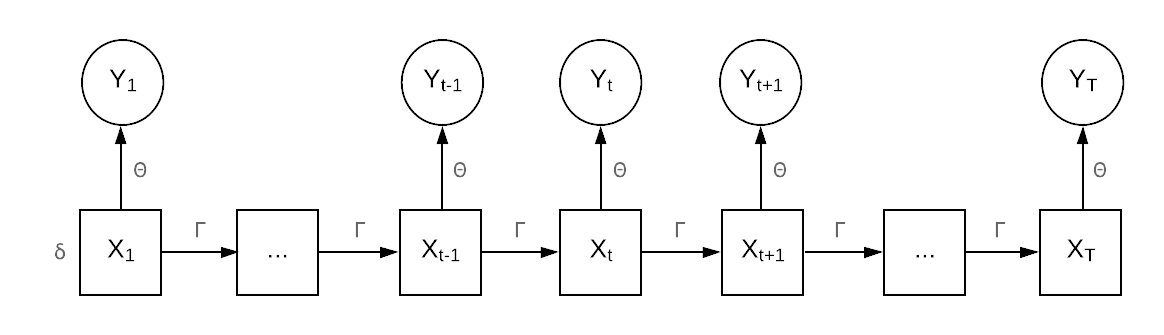
\includegraphics[width=4in]{../Plots/HMM.png}  
      \caption{Hidden Markov Model (\textbf{HMM})}
      \label{fig:HMM}
    \end{subfigure}
    %
    \newline
    %
    \begin{subfigure}{\textwidth}
      \centering
      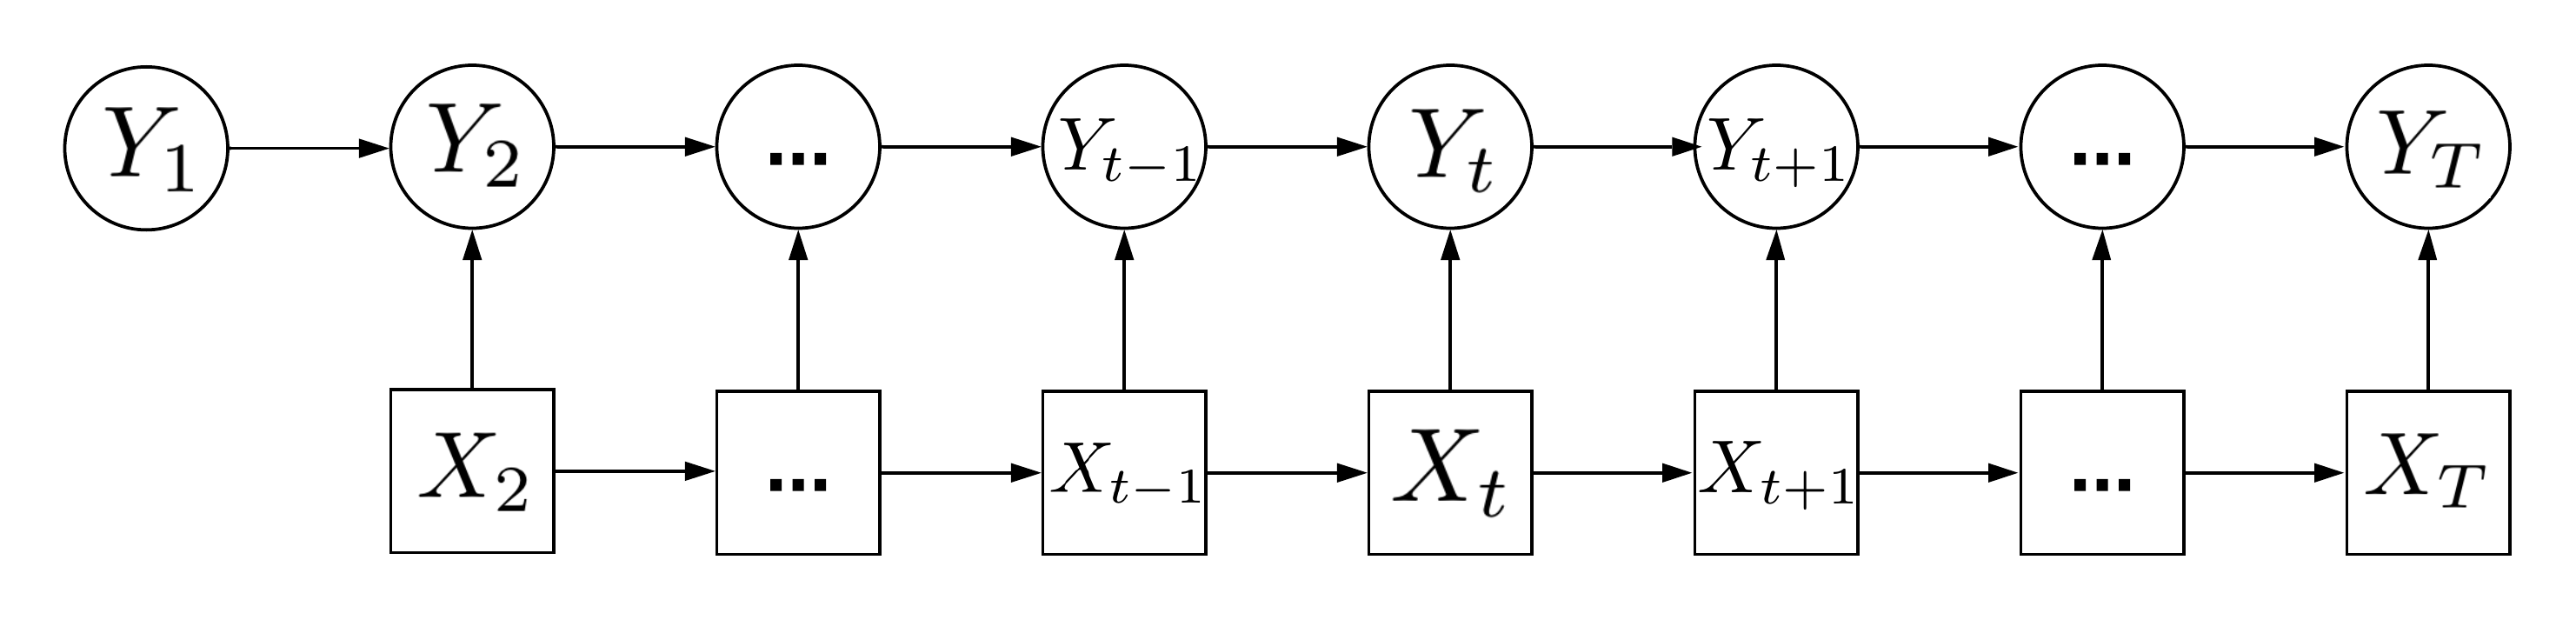
\includegraphics[width=4in]{../Plots/CarHMM.png}  
      \caption{Conditionally Autoregressive HMM (\textbf{CarHMM})}
      \label{fig:CarHMM}
    \end{subfigure}
    %
    \newline
    %
    \begin{subfigure}{\textwidth}
      \centering
      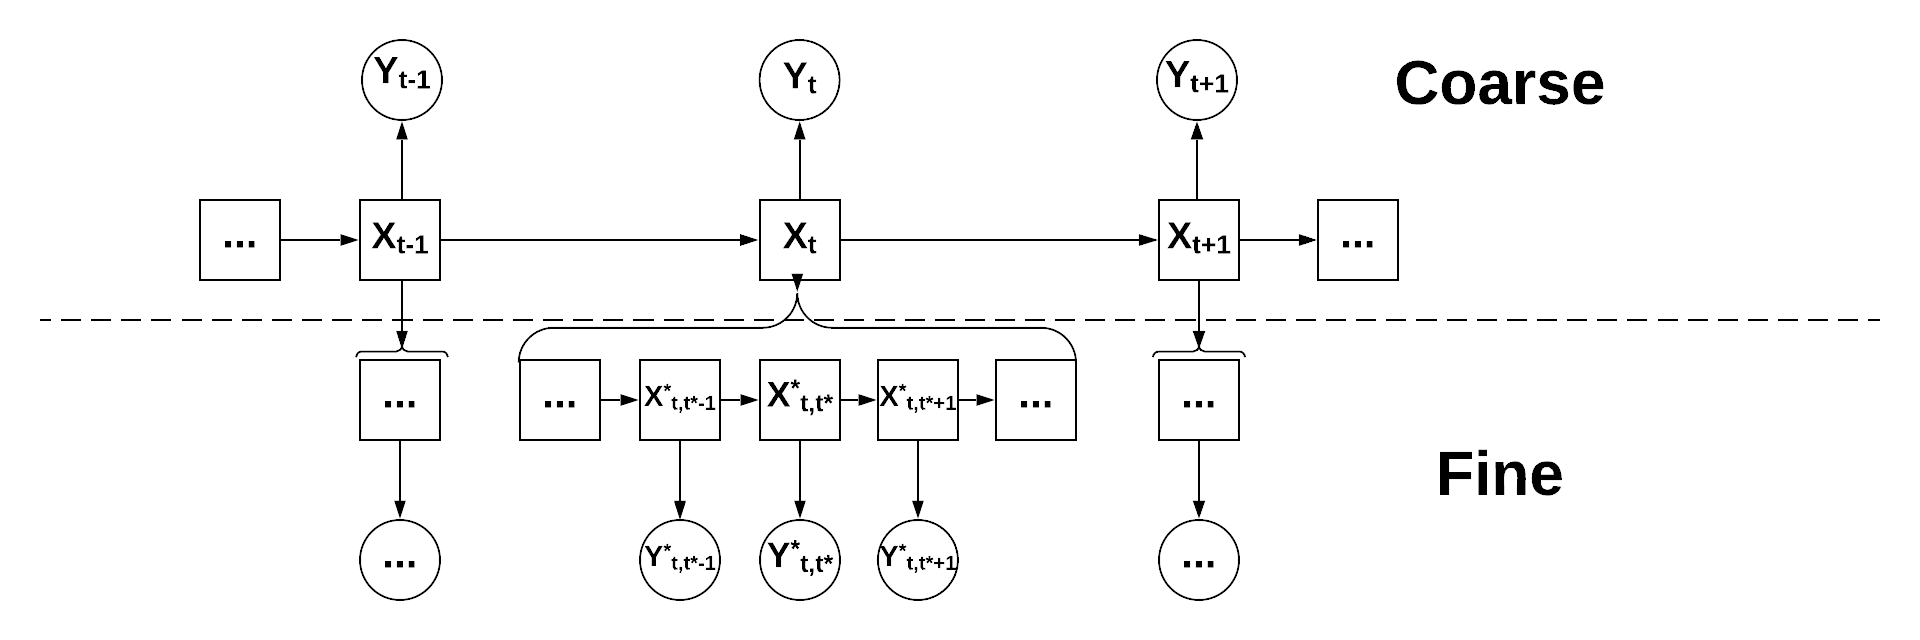
\includegraphics[width=4in]{../Plots/HHMM.png}  
      \caption{Hierarchical HMM (\textbf{HHMM})}
      \label{fig:HHMM}
    \end{subfigure}
    %
    \newline
    %
    \begin{subfigure}{\textwidth}
      \centering
      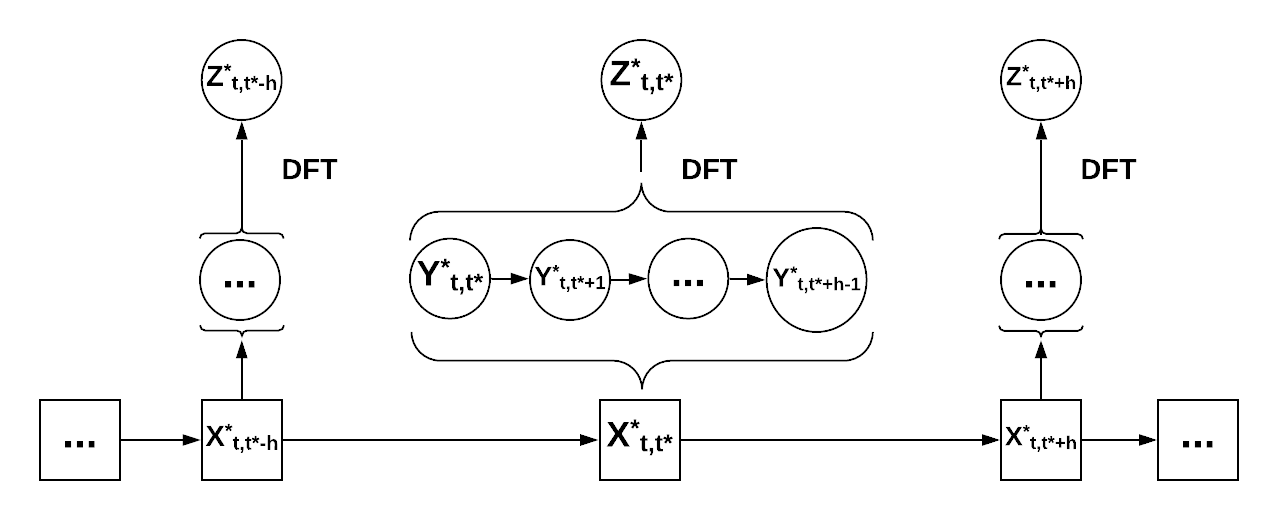
\includegraphics[width=4in]{../Plots/HMM-DFT.png}  
      \caption{HMM with Discrete Fourier Transform (\textbf{HMM-DFT})}
      \label{fig:HMM-DFT}
    \end{subfigure}
    \caption{Dependence structures of four HMM variants. Hidden state sequences are denoted as $X$ on the coarse-scale and $X^*$ at the fine scale. Observations (or emissions) are denoted by $Y$ on the coarse scale and $Y^*$ on the fine scale. Observations transformed using a moving window are denoted as $\Z$.}
    \label{fig:models}
\end{figure}

%%% data %%%

\begin{figure}[ht]
	\centering
	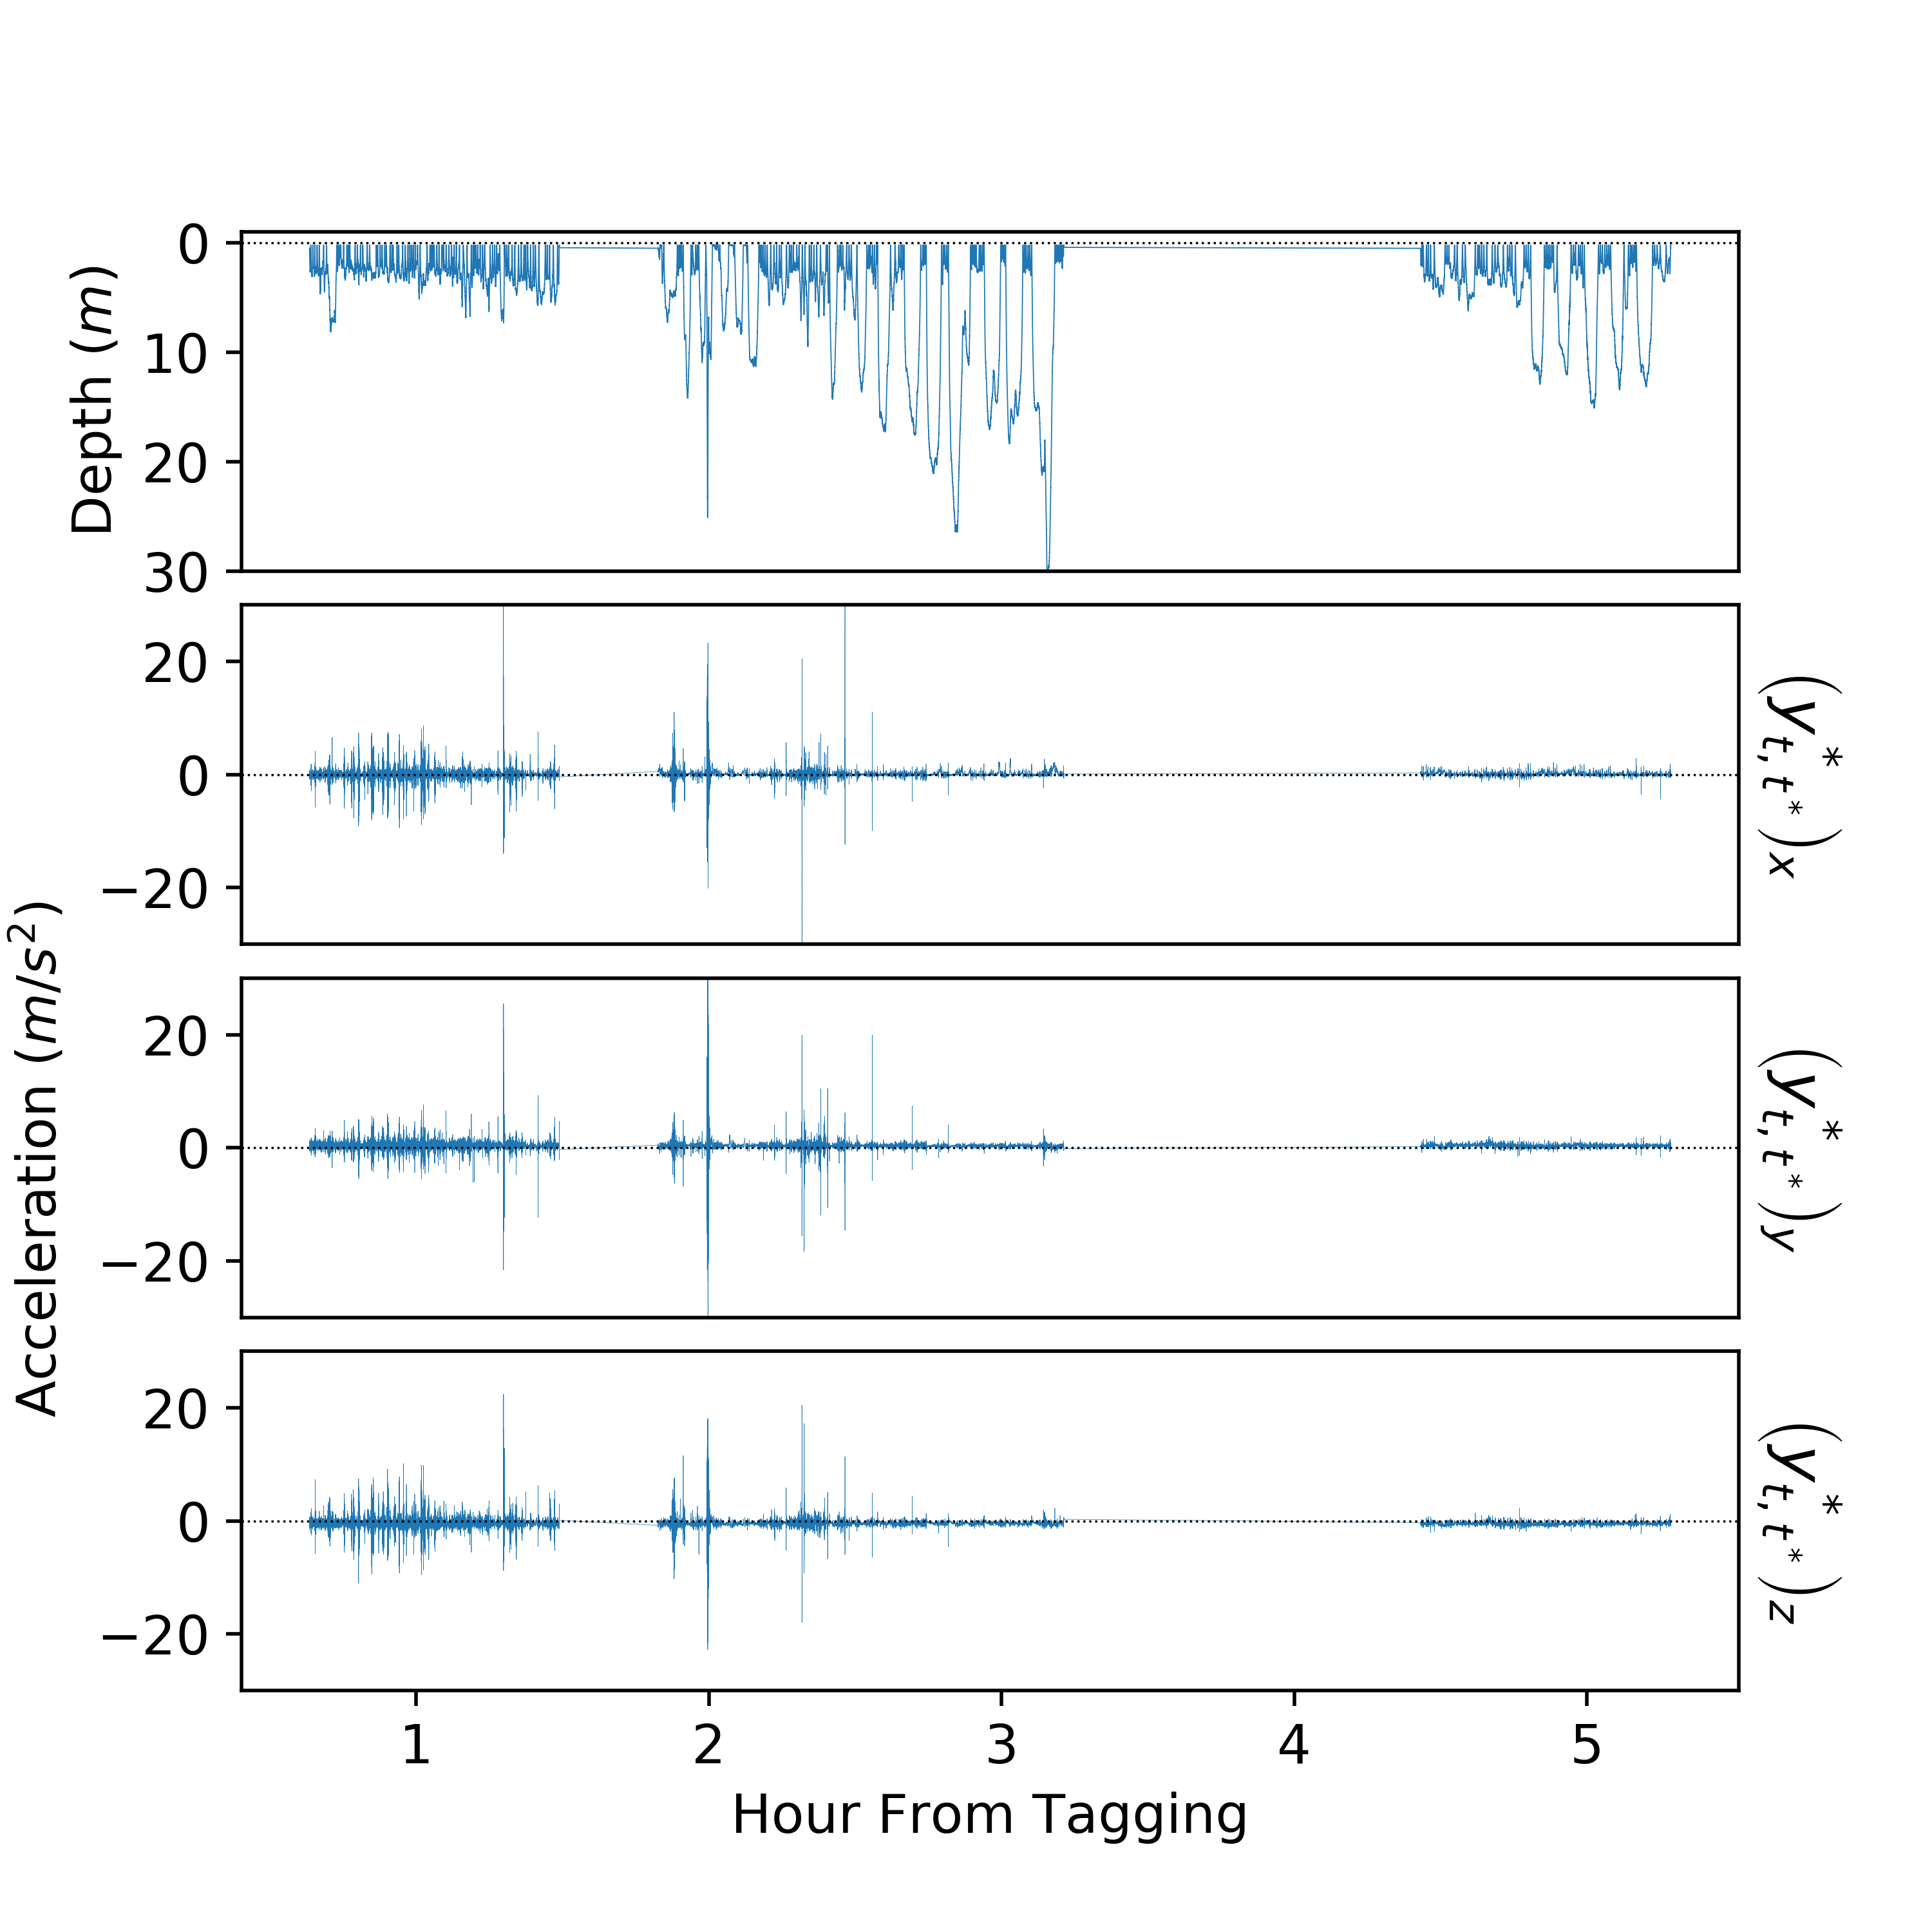
\includegraphics[width=5.25in]{../Plots/raw_data.png}
	\caption{Dive depth (top panel) and three-dimensional acceleration (bottom three panels) from a killer whale over approximately 5 hours. There are data gaps occurring from $\approx 1.5-1.8$ hours and from $\approx 3.2-4.5$ hours. Both data gaps were excluded from analyses.}
	\label{fig:data}
\end{figure}

\begin{figure}[ht]
	\centering
	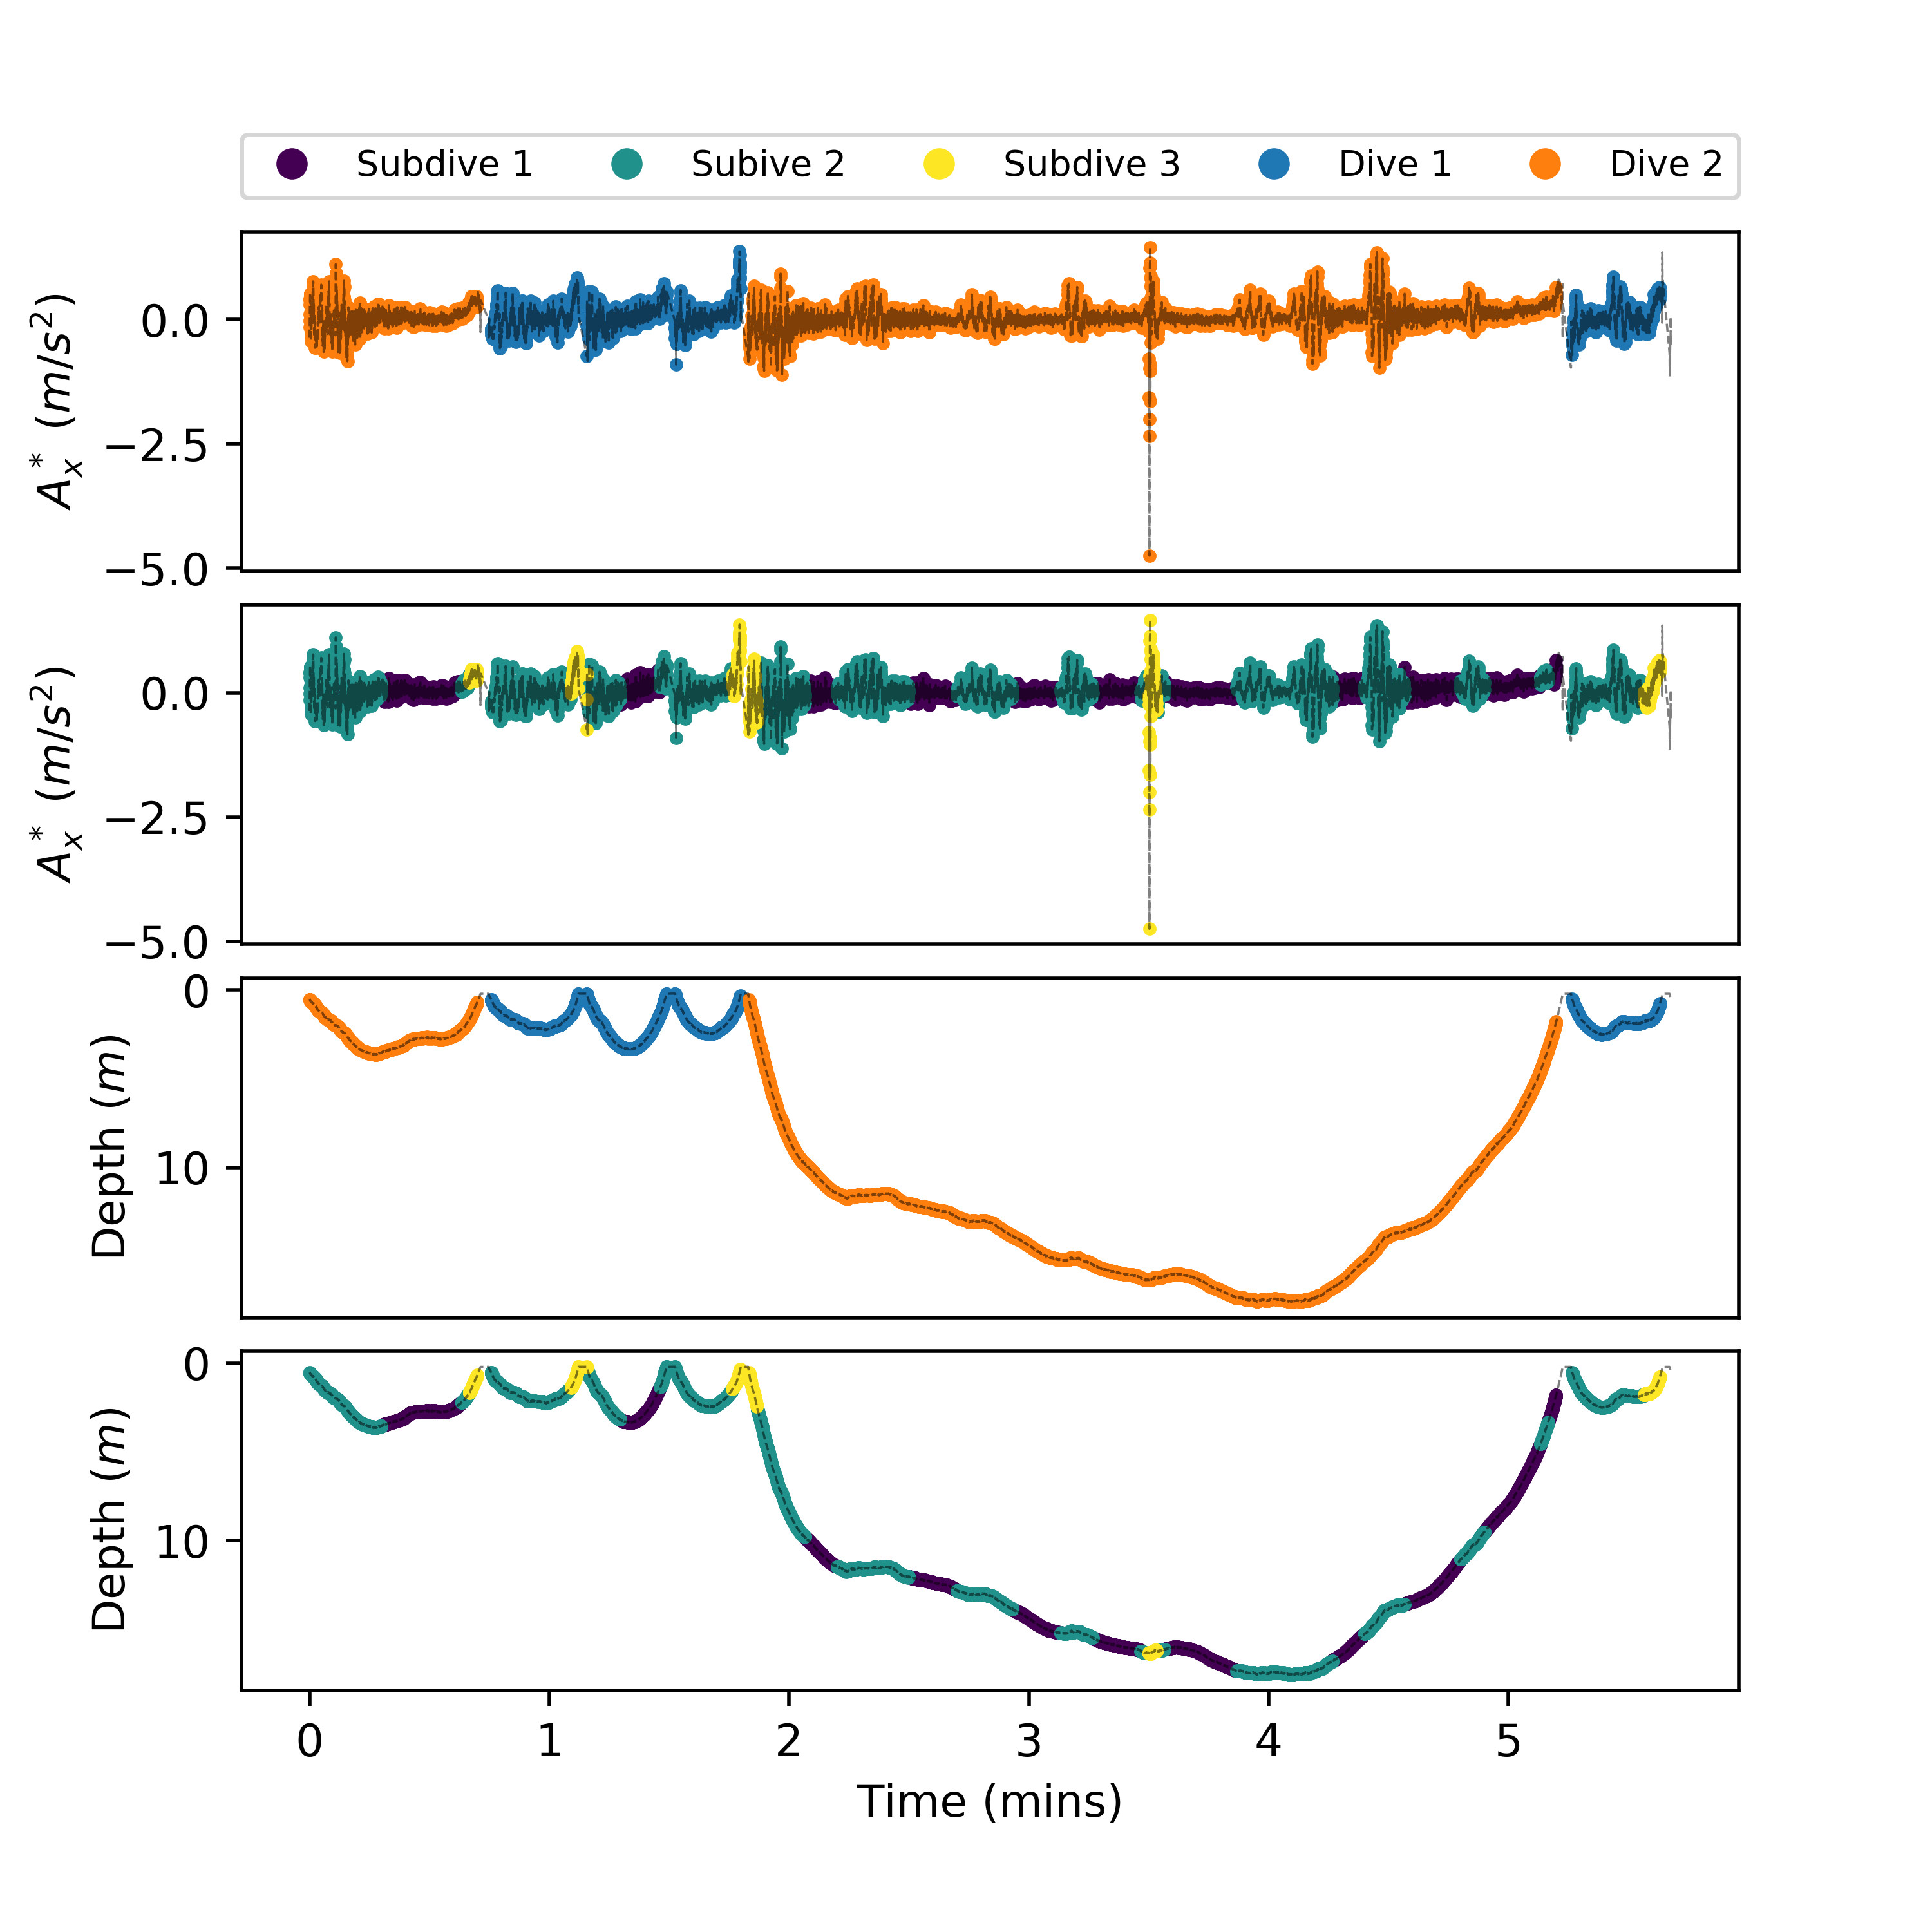
\includegraphics[width=5in]{../Plots/CarHHMM2_decoded_dives.png}
	\caption{The $x$-component of acceleration $\left(y^*_{t,t^*}\right)_x$ (top two panels) and dive depth (bottom two panels) of a northern resident killer whale for a sequence of six selected dives. The line colours in the first and third panels correspond to the estimated dive types while the line colours of the second and fourth panels correspond the estimated subdive states. Both the dive types and subdive states are estimated by fitting the CarHHMM-DFT to the data and performing the forward-backward algorithm to determine the hidden state with the highest probability.}
	\label{fig:labeled_dives}
\end{figure}

%%% Case Study %%%

\begin{figure}[ht]
	\centering
	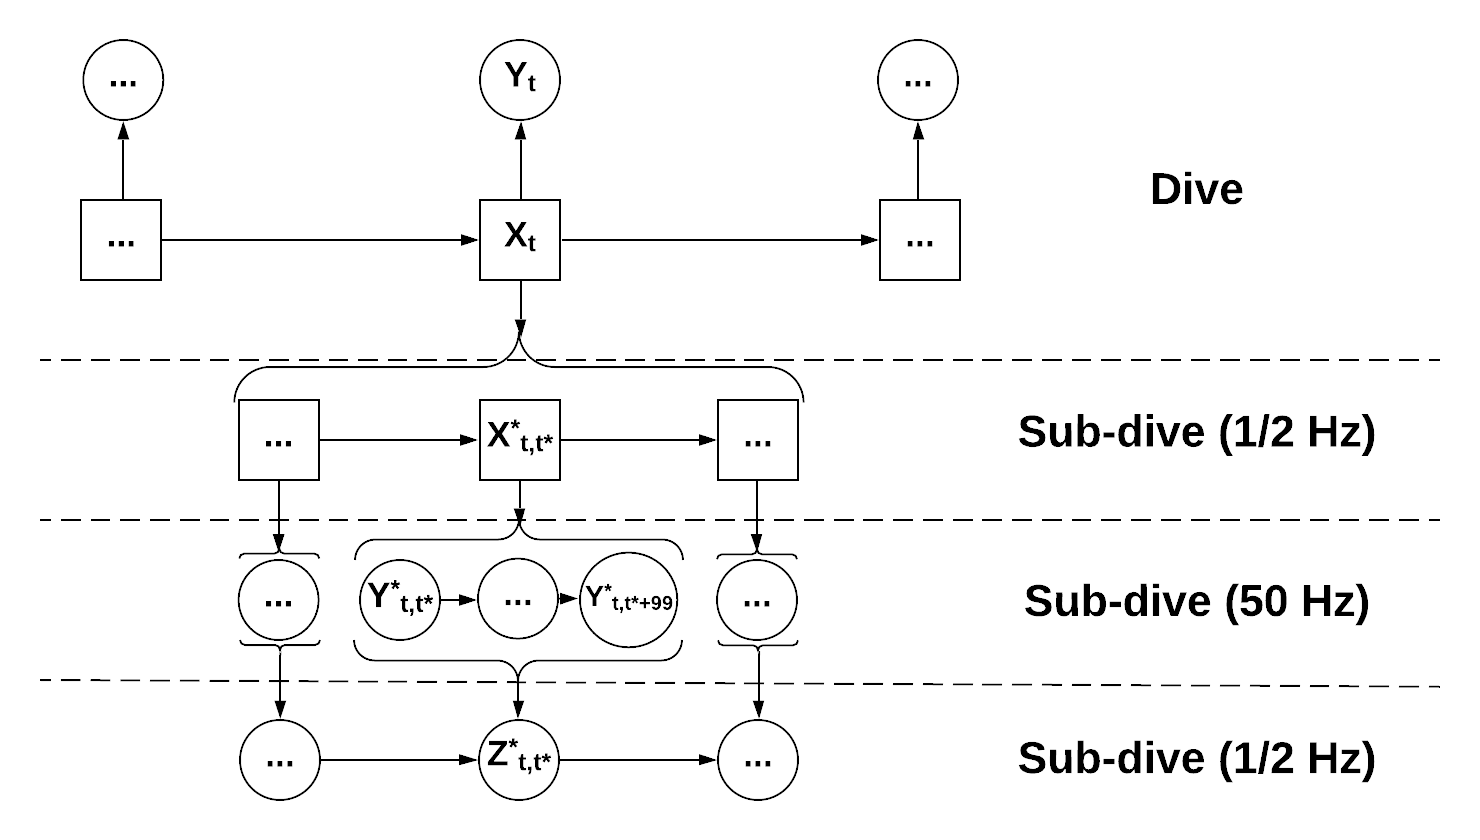
\includegraphics[width=5in]{../Plots/CarHHMM-DFT.png}
	\caption{Graphical representation of the conditionally auto-regressive hierarchical hidden Markov model with discrete Fourier transform \textbf{CarHHMM-DFT} used in the killer whale simulation and case study. The type of dive $t$ is denoted by $X_t$ and $Y_t$ represents the associated dive duration. The raw acceleration vector associated with dive $t$ and time stamp $t^*$ is denoted by $Y^*_{t,t^*}$. The subdive state of the killer whale during dive $t$ and window $\tilde t^*$ is denoted as $\tilde X^*_{t,\tilde t^*}$, and the corresponding transformed observations are denoted by $\Z_{t,\tilde t^*}$.}
	\label{fig:CarHHMM-DFT}
\end{figure}

\begin{figure}[ht]
	\centering
	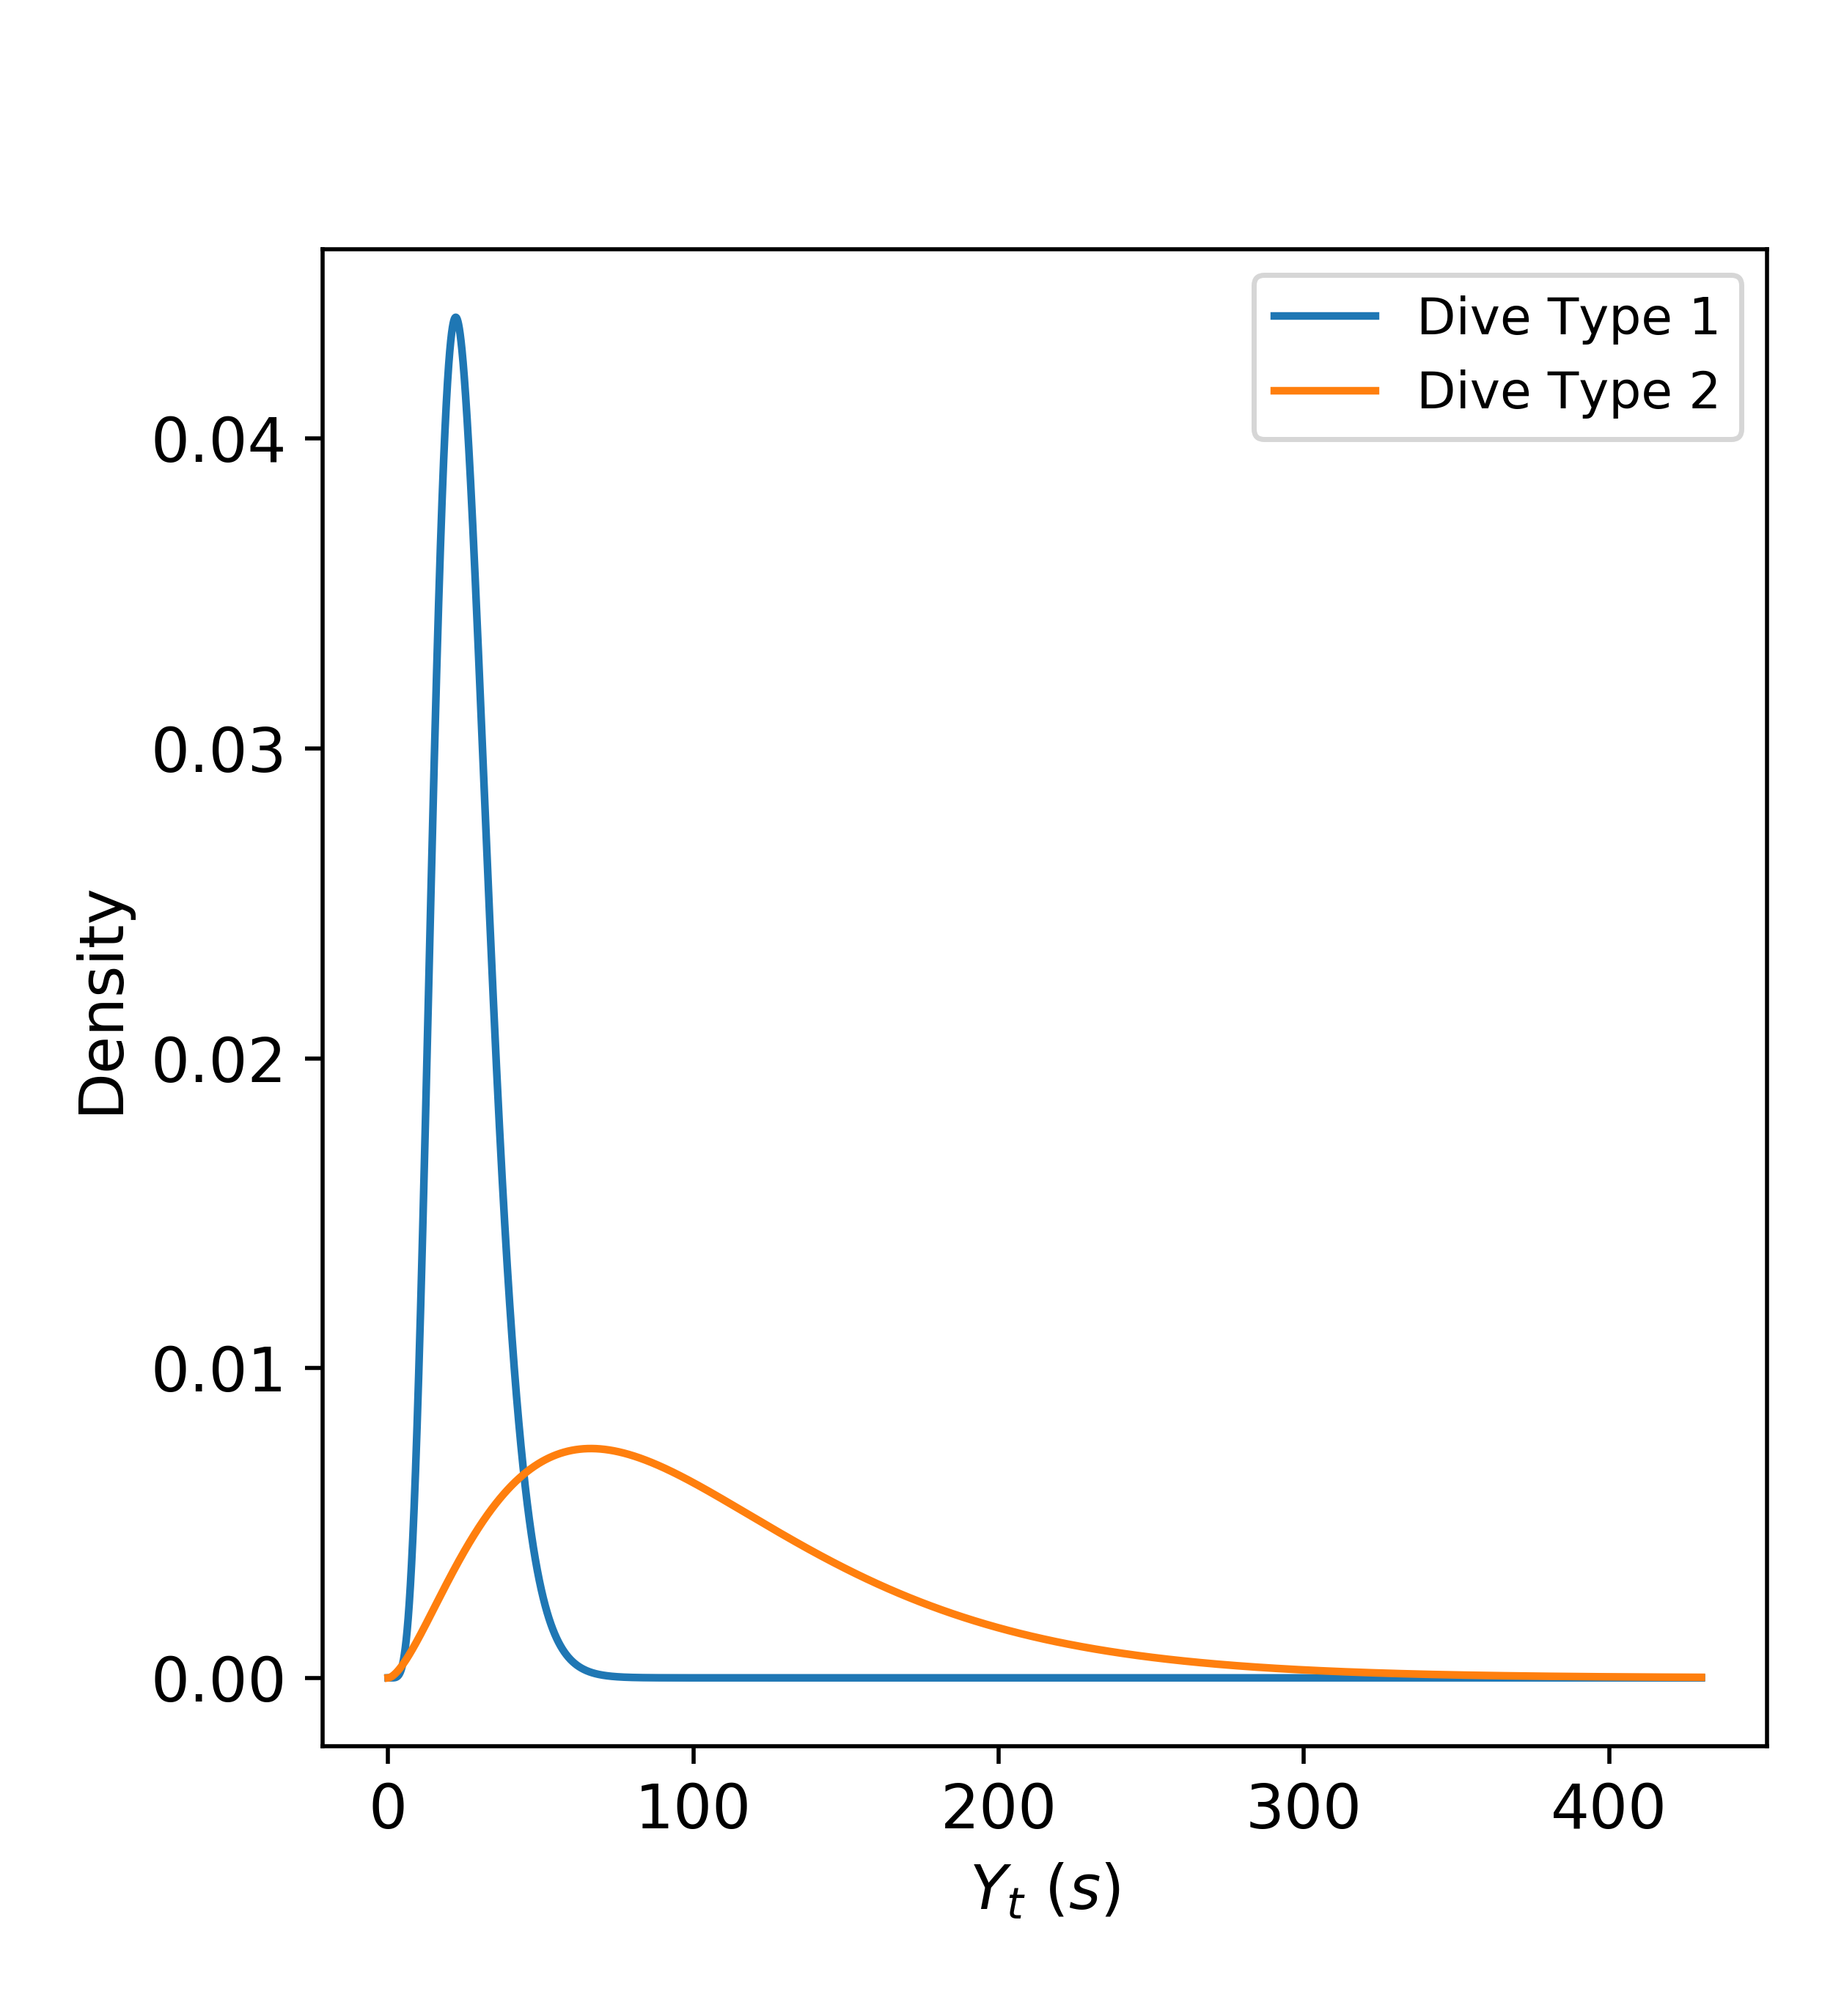
\includegraphics[width=5in]{../Plots/CarHHMM2-coarse-emissions.png}
	\caption{Estimated Gamma probability density functions of dive duration ($Y_t$) corresponding to dive types 1 (short dives) and dive type 2 (longer dives). These  densities are used to characterize the behaviour of a killer whale and are found by fitting the CarHHMM-DFT to the killer whale case study data.}
	\label{fig:coarse_emis}
\end{figure}

\begin{figure}[ht]
	\centering
	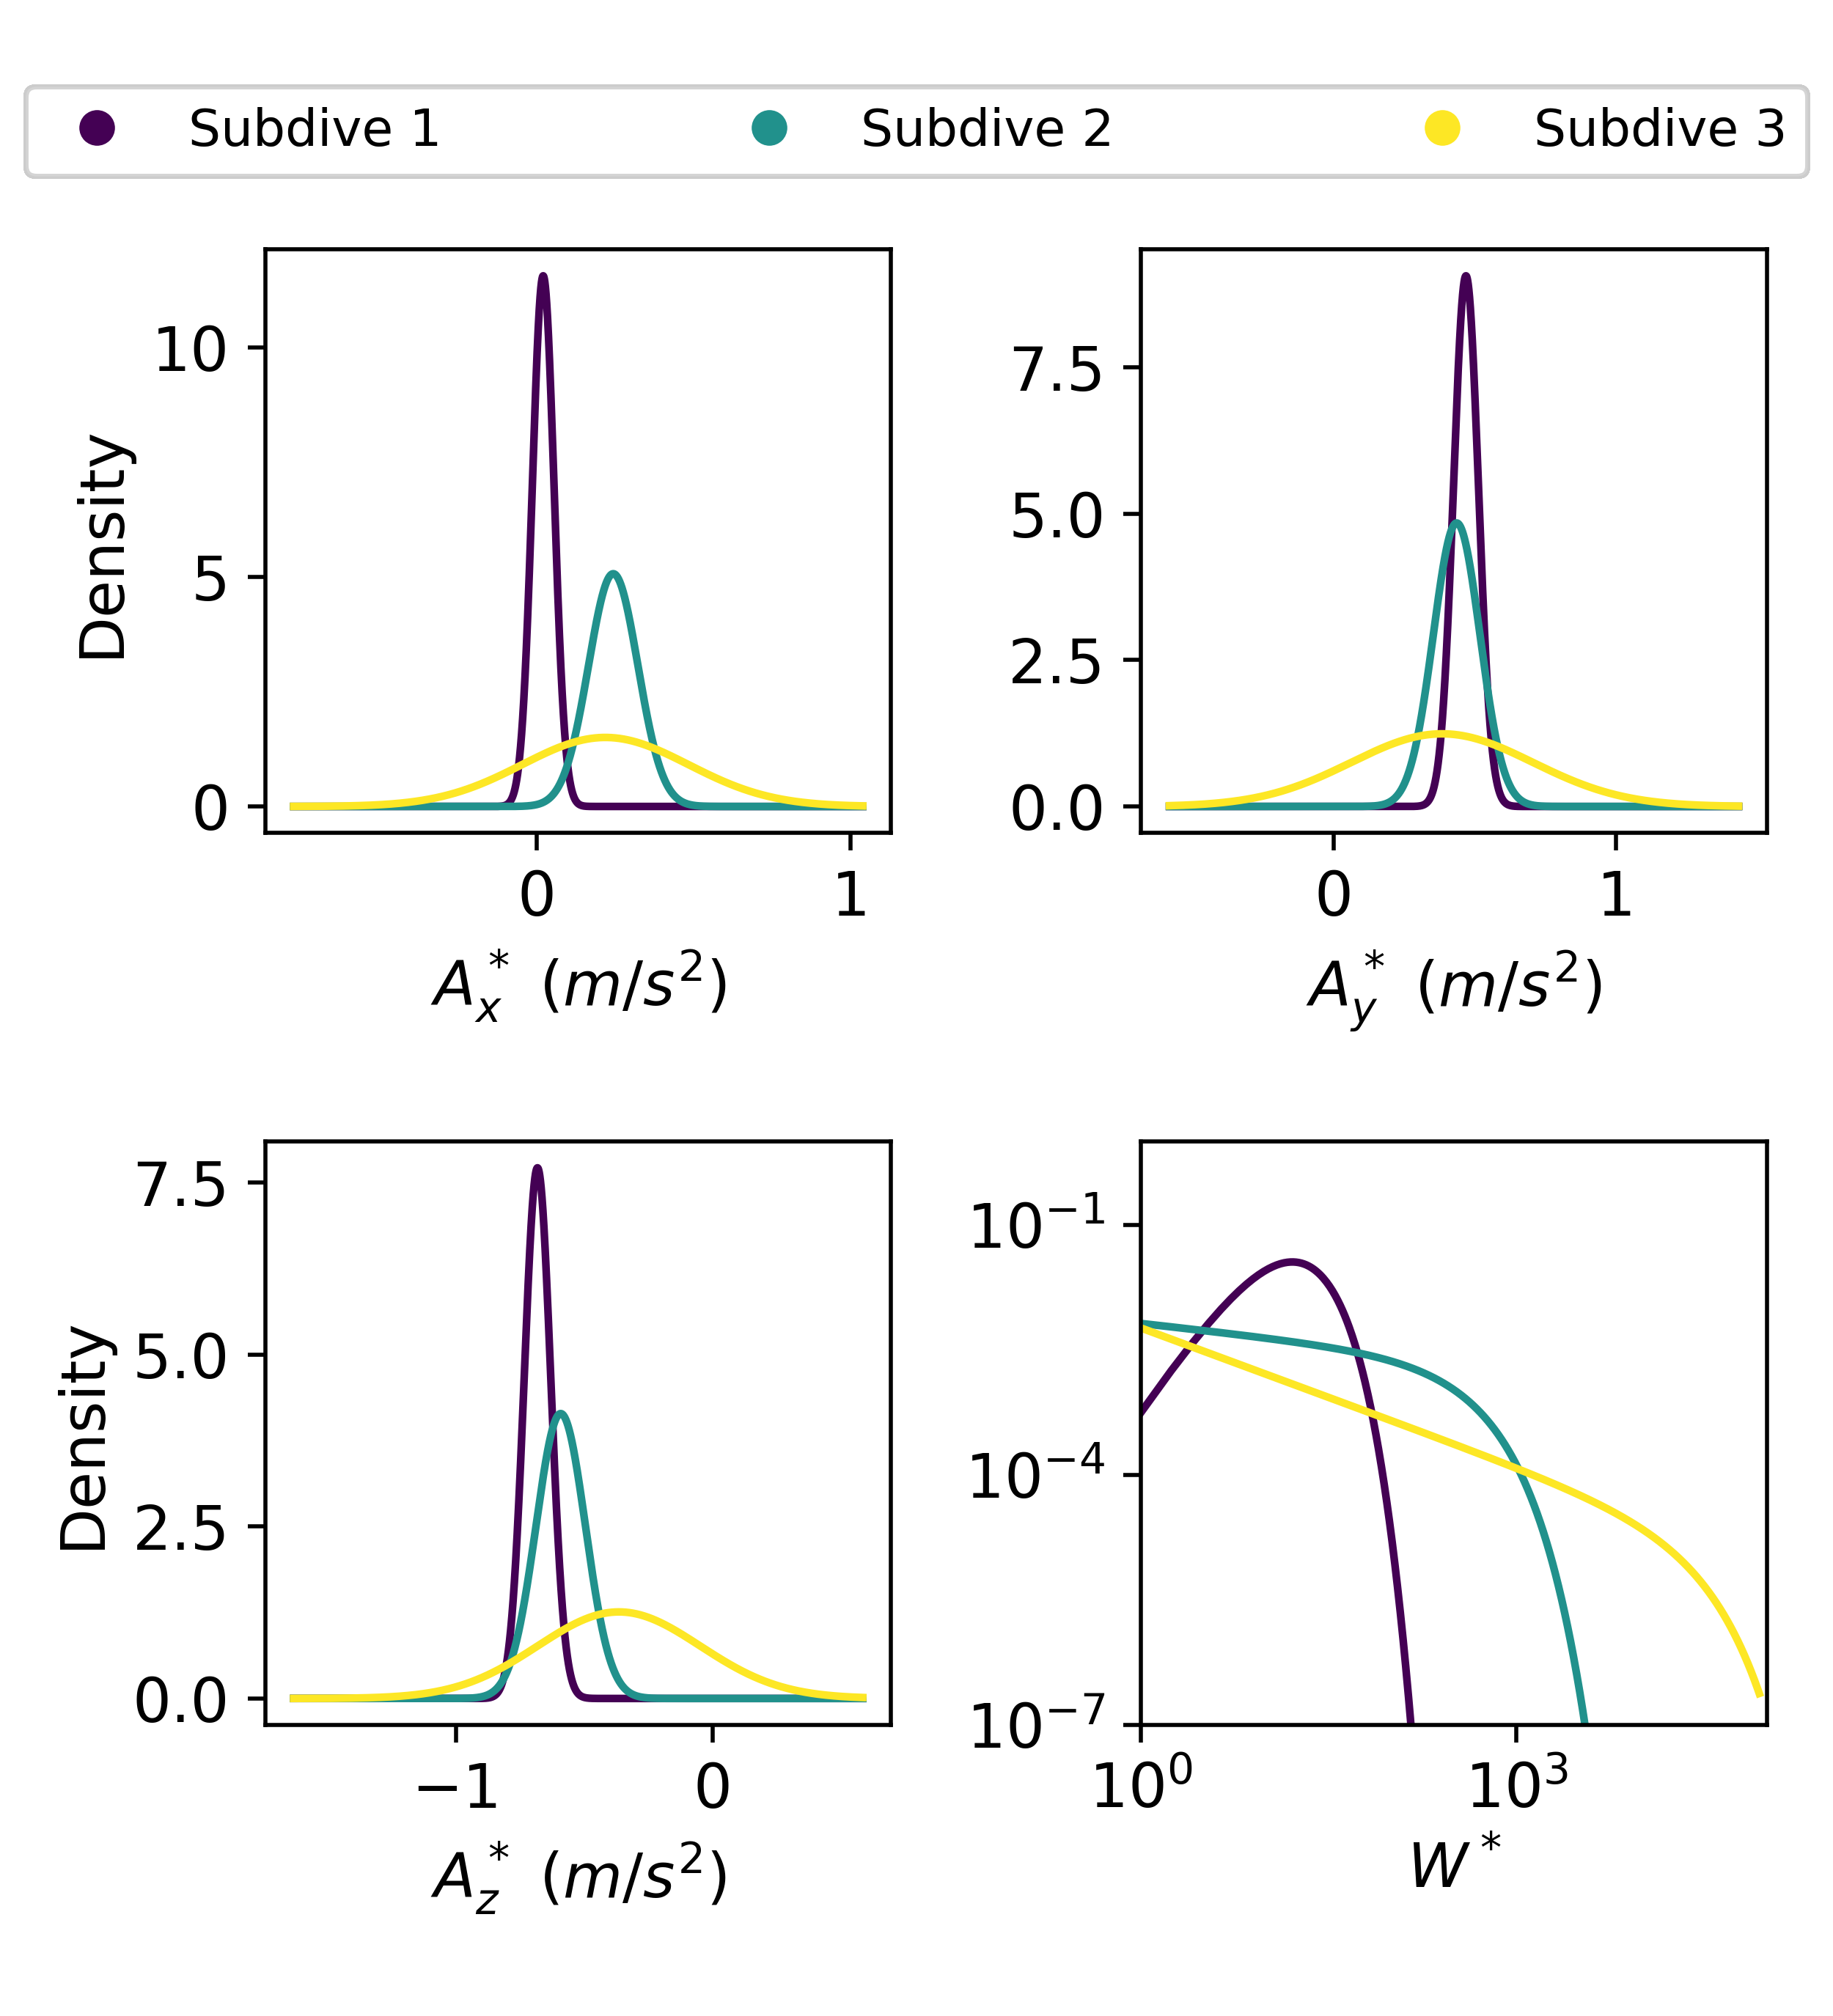
\includegraphics[width=5in]{../Plots/CarHHMM2-fine-emissions.png}
	\caption{Estimated probability density of wiggliness ($\Ztwo_{t,\tilde t^*}$) and estimated conditional density of acceleration ($\Zone_{t,\tilde t^*}|\Zone_{t,\tilde t^*-1} = \mu_A^{*(\cdot,i^*)}$) corresponding to subdive states $i^* = 1,2,3$ of a killer whale (see Table \ref{table:emis_dists_CarHHMM-DFT}). The estimated conditional density of acceleration is Normal and plotted on a linear scale while the estimated density of wiggliness is Gamma and plotted on a log-log scale.}
	\label{fig:fine_emis}
\end{figure}

\begin{figure}[ht]
    \begin{subfigure}{0.45\textwidth}
    	\centering
    	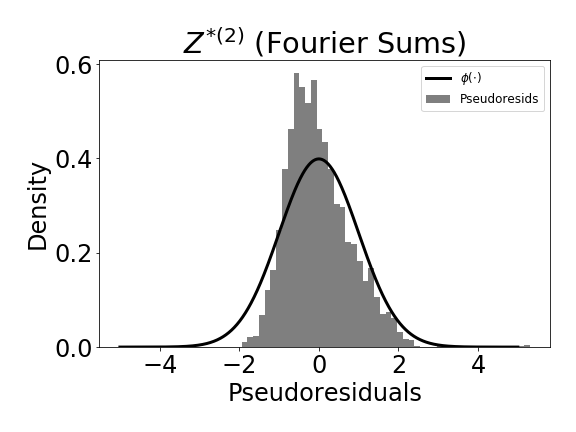
\includegraphics[width=2.25in]{../Plots/CarHHMM2_psedoresids_ahat.png}
    	\caption{Histogram of pseudoresiduals of $\tilde W^*_{t,\tilde t^*}$}
    	\label{fig:pseudoresids}
    \end{subfigure}
    \begin{subfigure}{0.45\textwidth}
    	\centering
    	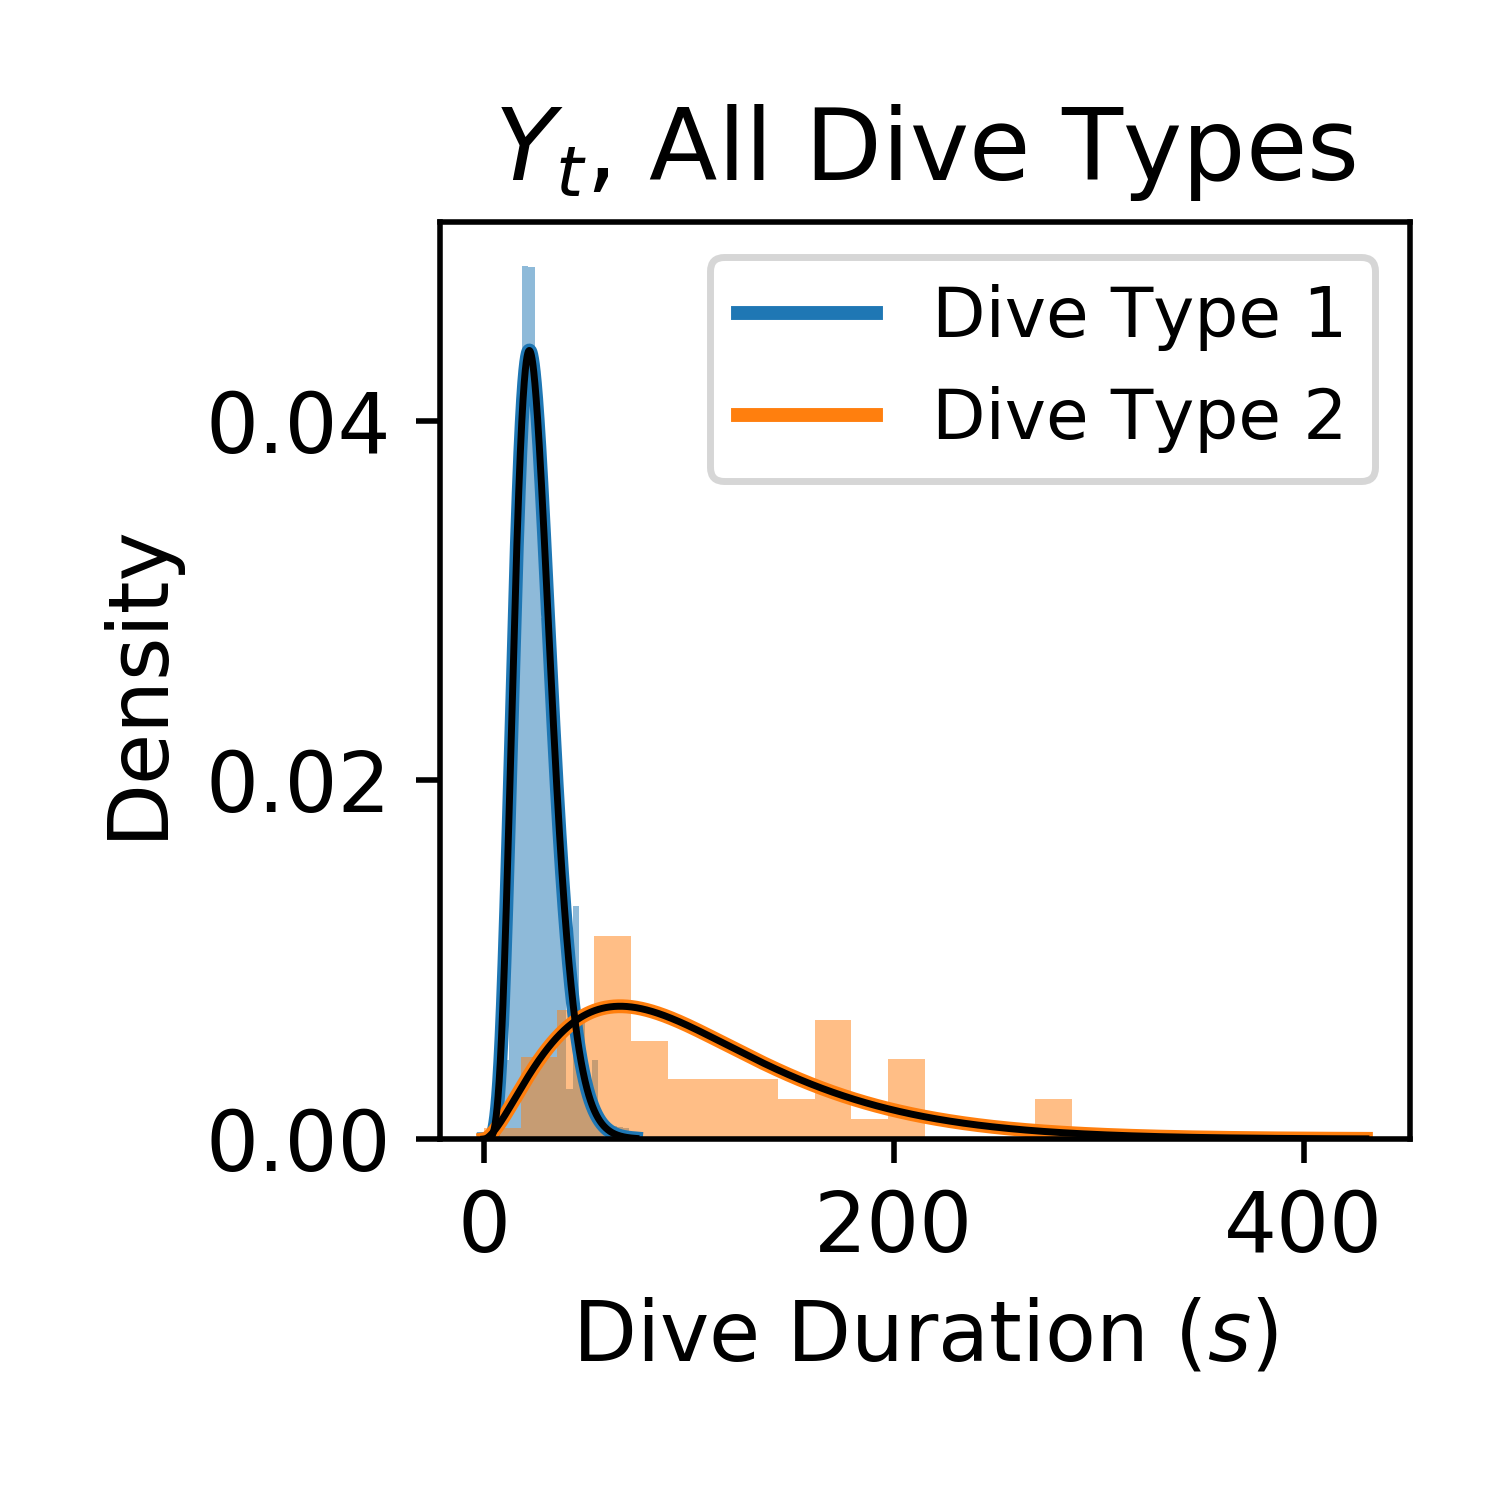
\includegraphics[width=2.25in]{../Plots/CarHHMM2_empirical_hist_dive_duration.png}
    	\caption{Empirical distribution of $Y_t$}
    	\label{fig:empirical_dist}
    \end{subfigure}
    \caption{Pseudoresiduals of wiggliness ($\Phi^{-1} \left(Pr(\Ztwo_{t,\tilde t^*} < \ztwo_{t,\tilde t^*}|Y,\tilde Y^* / \{\Ztwo_{t,\tilde t^*}\}) \right)$ , left) plotted over a standard normal density as well as a weighted empirical distribution of dive duration ($Y_t$, right) plotted over the corresponding fitted Gamma distributions. Both plots are generated by fitting the CarHHMM-DFT to the killer whale case study data and performing the forward-backward algorithm.}
    \label{fig:model_checking}
\end{figure}

%%% simulation study %%%

\begin{figure}[ht]
	\centering
	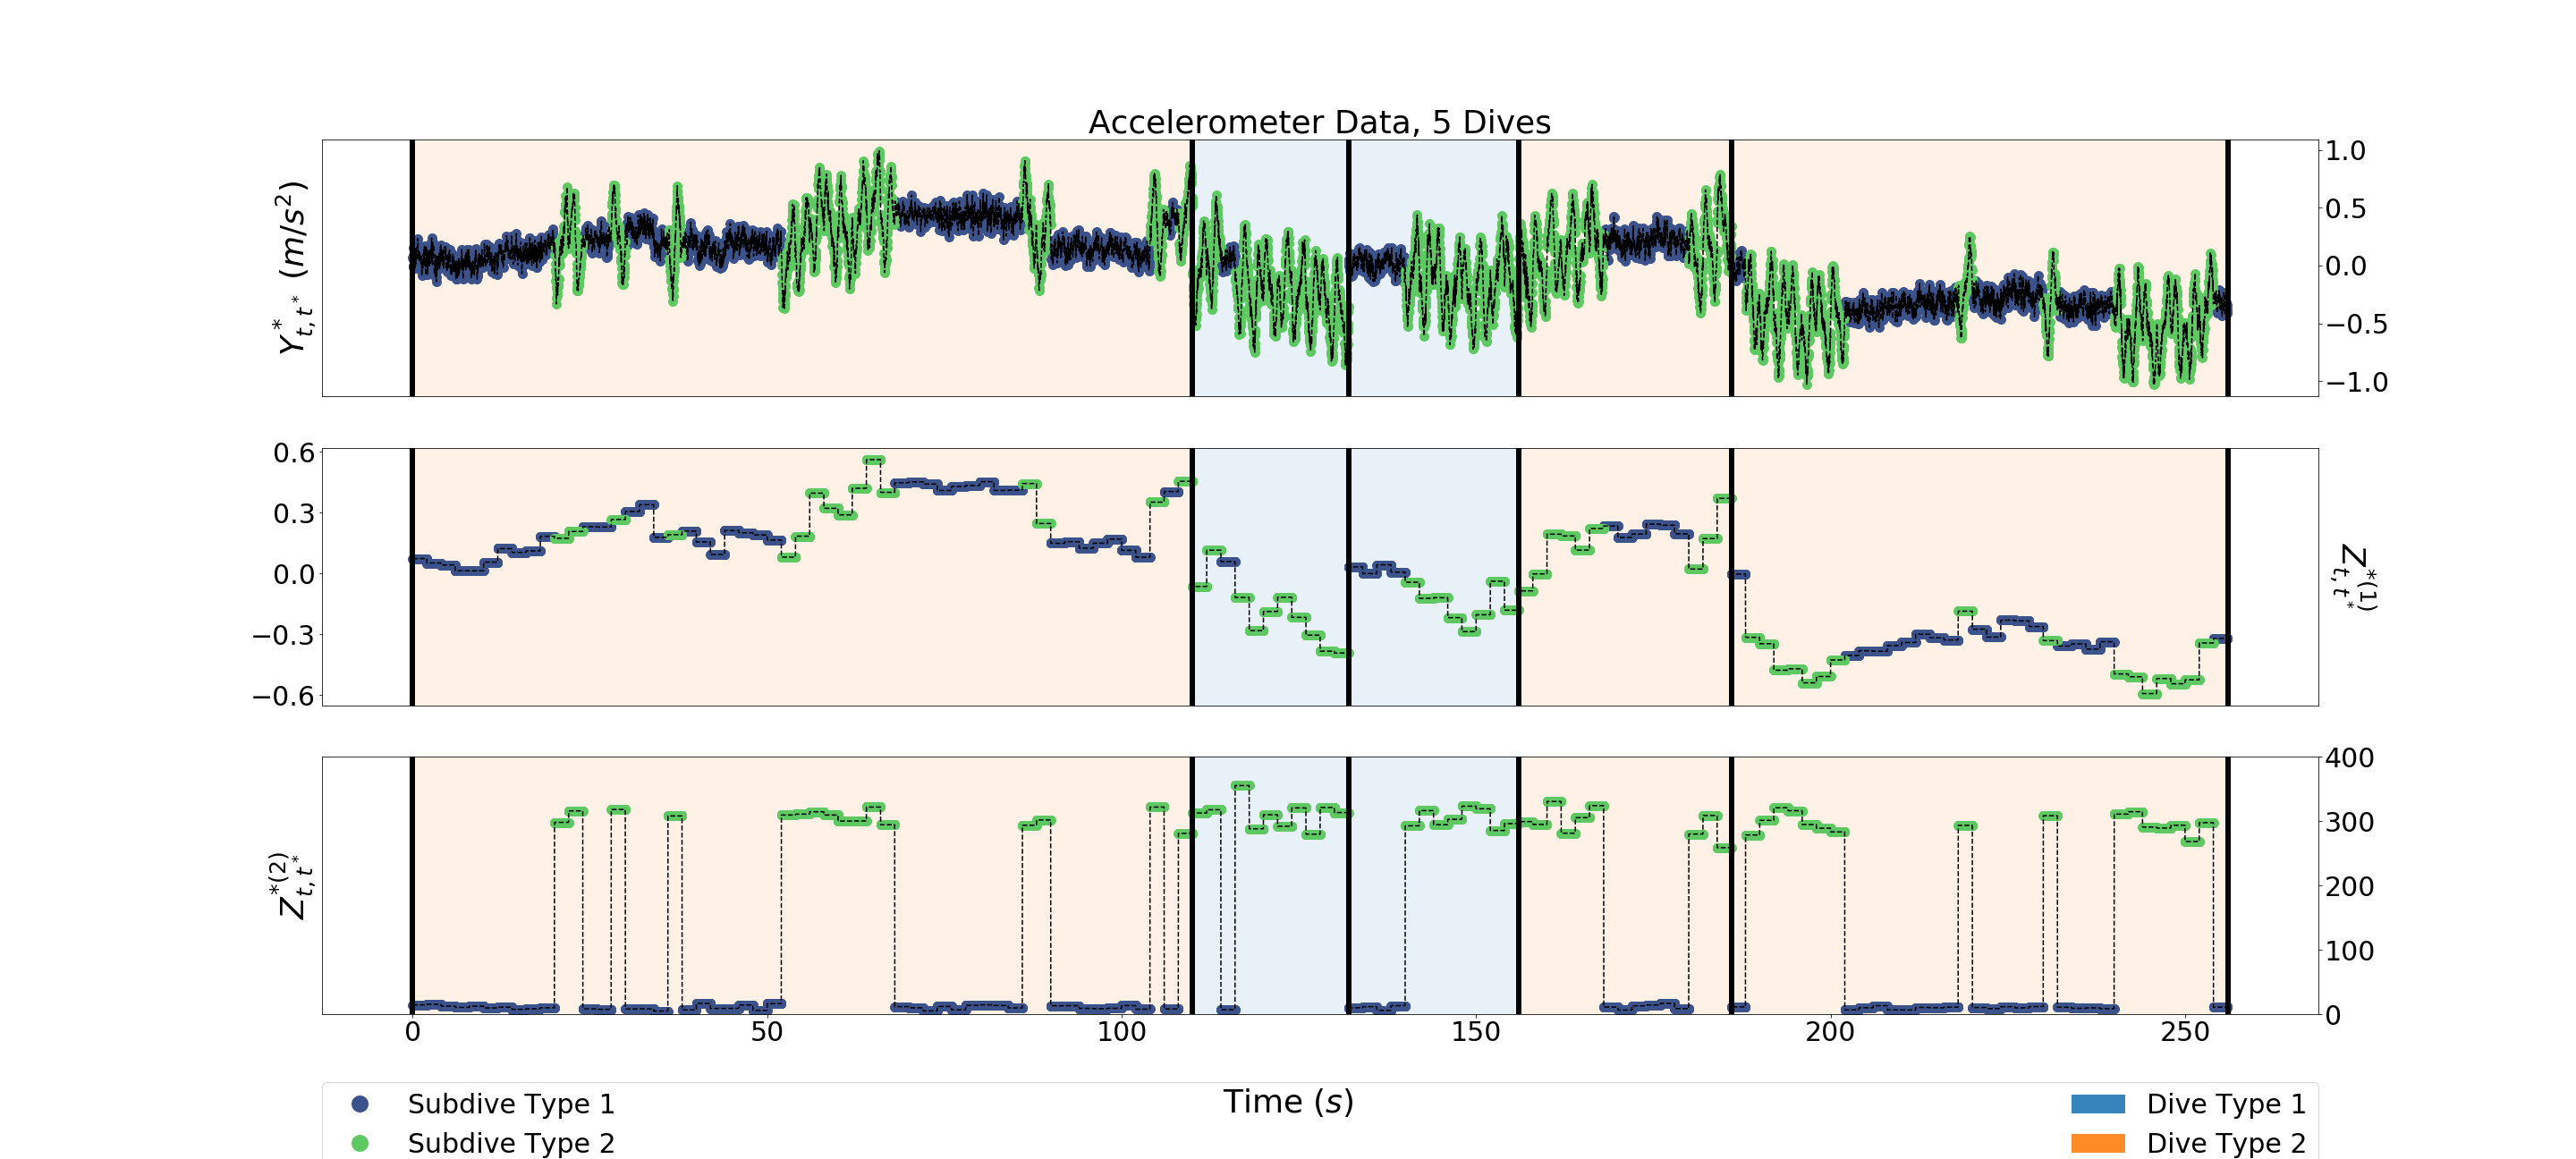
\includegraphics[width=5in]{../Plots/sim_data.png}
	\caption{Acceleration data for a single dive of a selected simulated data set. The raw accelerometer data is denoted as $Y^*_{t,\tilde t^*}$ which is recorded at 50 hertz while $\Zone_{t,\tilde t^*}$ and $\Ztwo_{t,\tilde t^*}$ are recorded at 0.5 hertz. The colour of the line corresponds to the true fine-scale state, while the colour of the background corresponds to the true dive type. Subdive state 1 can plausibly be interpreted as ``gliding" while subdive state 2 can plausibly be interpreted as active swimming, or ``fluking".}
	\label{fig:sim_data}
\end{figure}

\begin{figure}[ht]
    \centering
    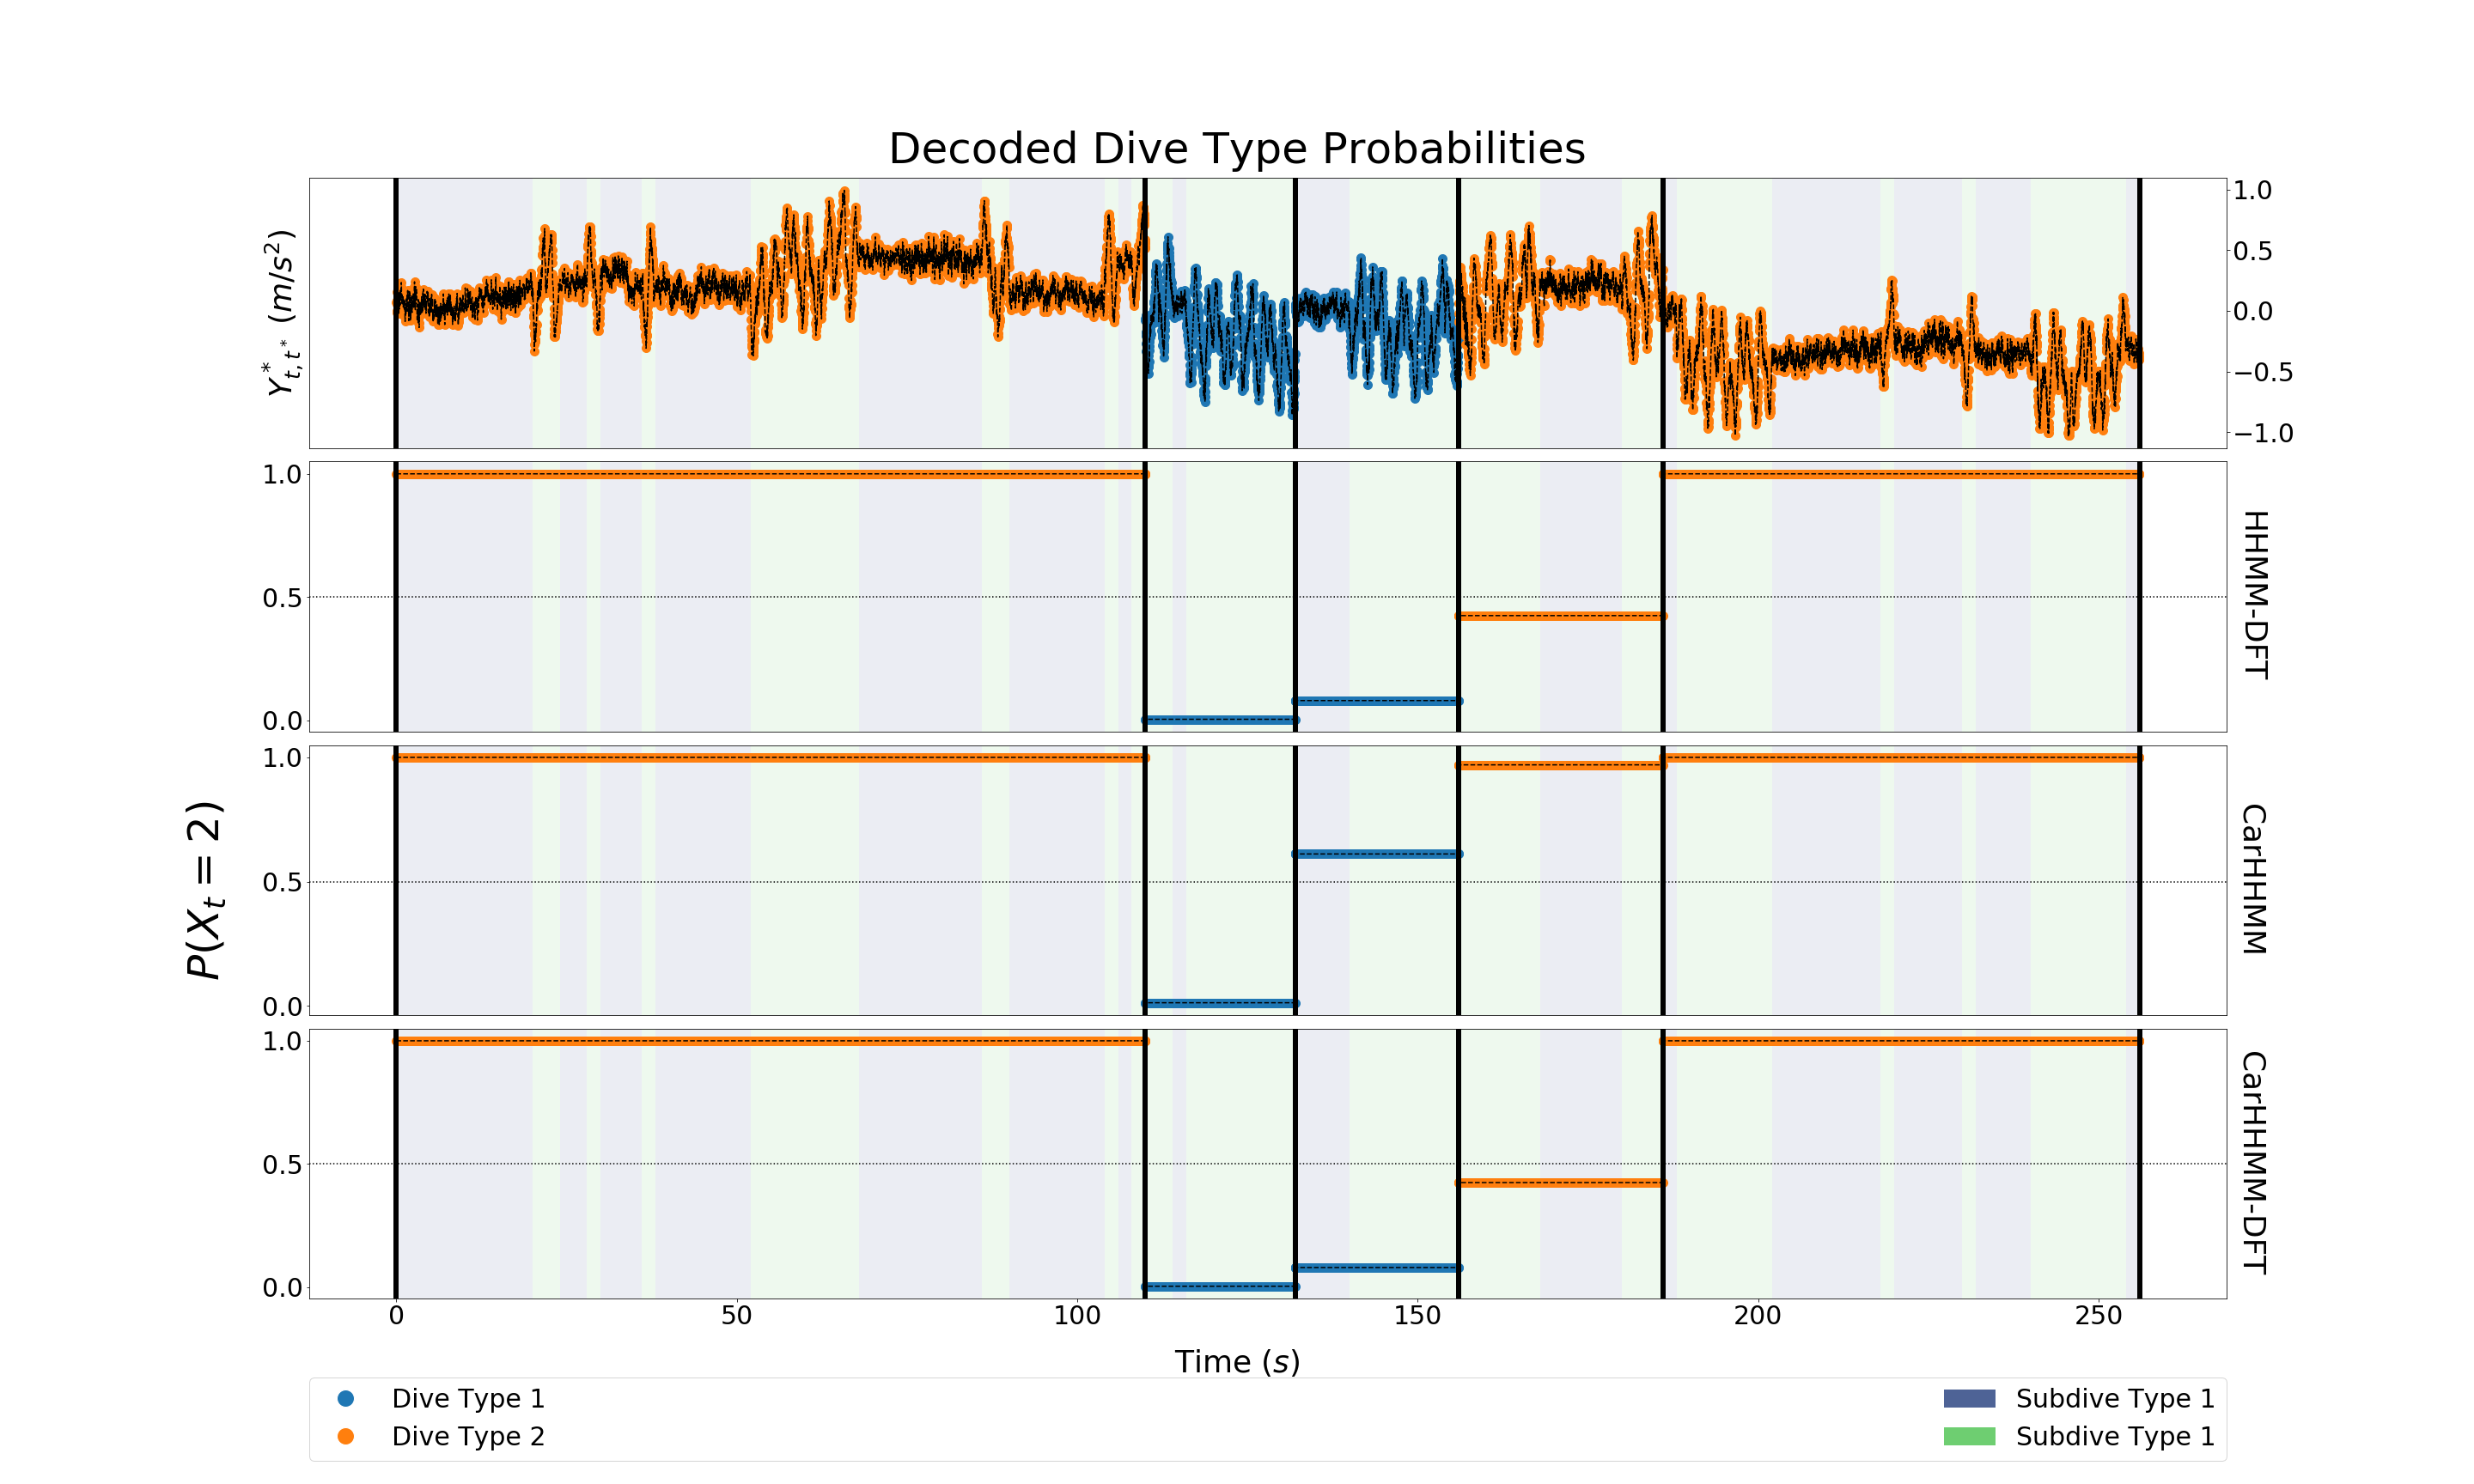
\includegraphics[width=4.5in]{../Plots/Posterior_Coarse_States.png}
    \caption{Estimated probabilities that each dive is of type two for five selected dives of one simulated data set. The colour of the line corresponds to the true dive type while the colour of the background corresponds to the true subdive state. The CarHMM-DFT is omitted because it incorporates only one dive type.}
    \label{fig:acc_coarse}
\end{figure}

\begin{figure}[ht]
    \centering
    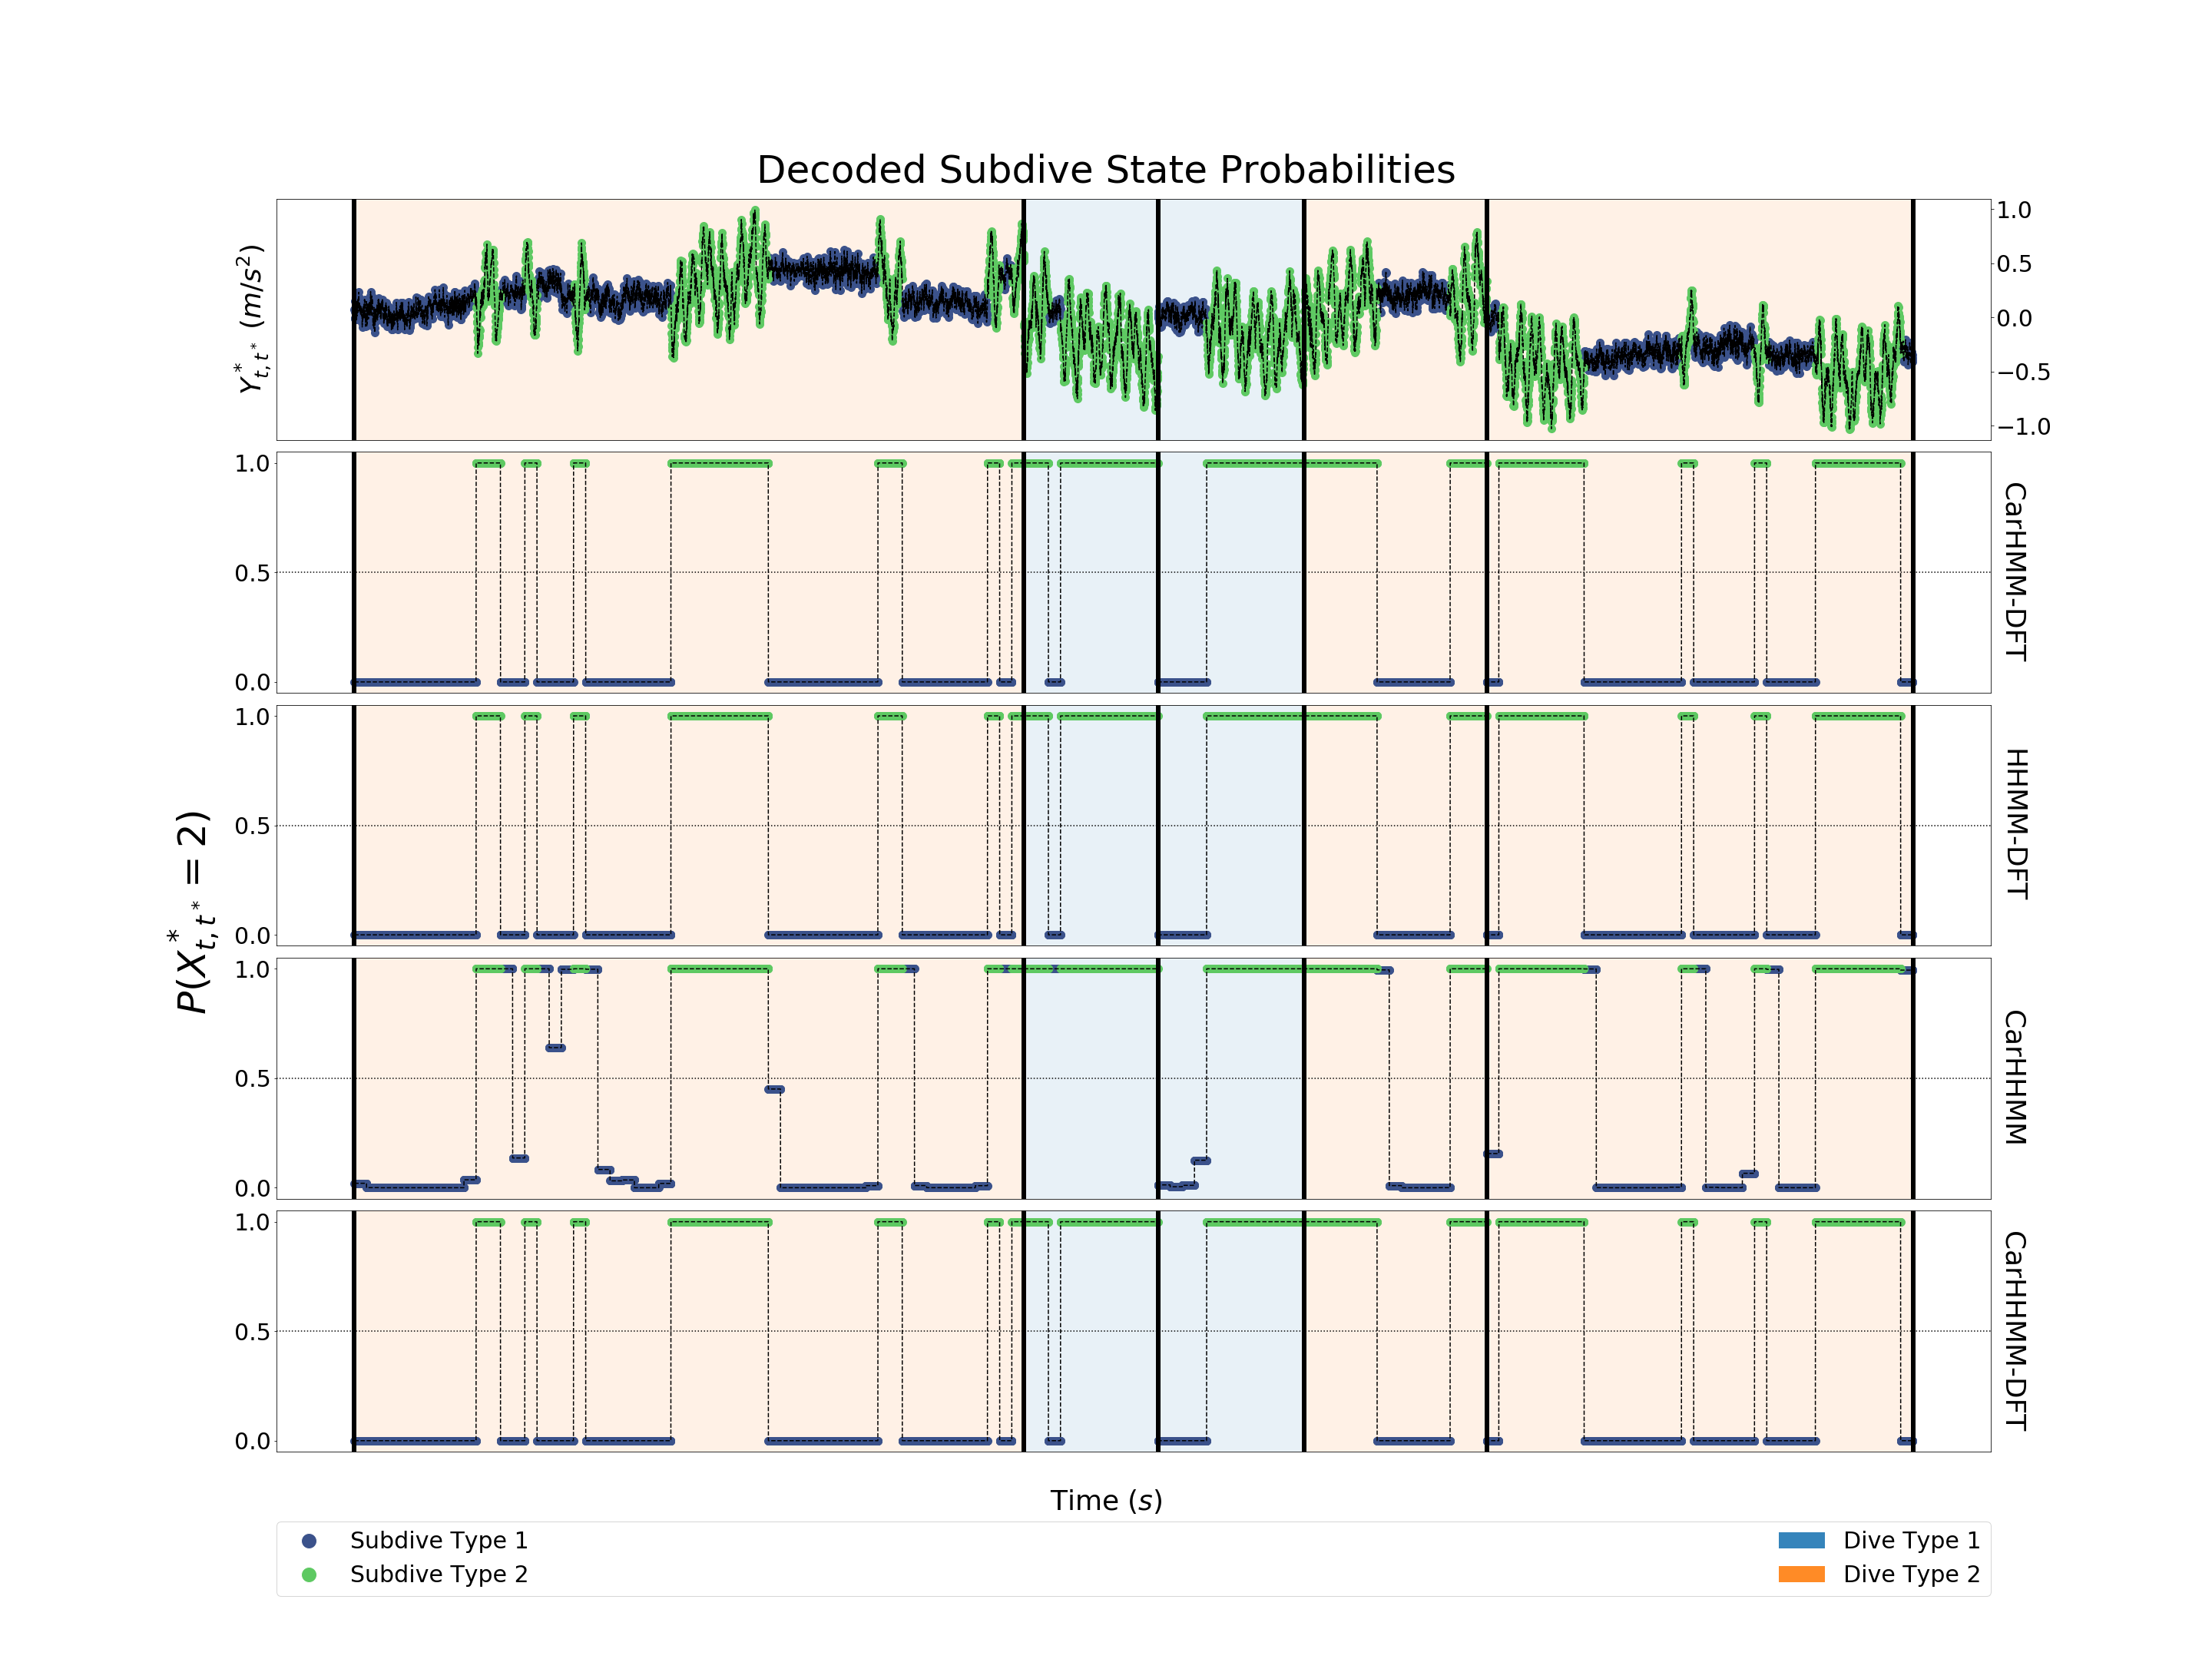
\includegraphics[width=4.5in]{../Plots/Posterior_Fine_States.png}
    \caption{Estimated probabilities that each window corresponds to subdive state two for five selected dives of one simulated data set. The colour of the line corresponds to the true subdive state while the colour of the background corresponds to the true dive type.}
    \label{fig:acc_fine}
\end{figure}